\begin{frame} %%% DEM
\frametitle{Discrete Euler-Maruyama (DEM)}
Method:
\begin{equation*}
	\left \{
	\begin{aligned}
		X_{h,i+1}^d &= f(X_{h,i}^d)h + g(X_{h,i}^d)(W(t_{i+1}) - W(t_{i})),  \\
		X_{h,0}^d &= X_0.
	\end{aligned} \right .
\end{equation*}
Parameters of interest computed naively
\begin{equation*}
\begin{aligned}
	\tau_h^d &= \min\{\tau_{h,e}^d,T\}, \text{ where } \tau_{h,e}^d = h\min \{i \colon X_{h,i}^d \notin D\}. \\
	 \phi_h^d &= \mathbbm{1}_{\{T < \tau_{h,e}^d\}}F(X_{h,N}^d).
\end{aligned}
\end{equation*}
Missed exits $\to$ 1/2 loss in weak order:
\begin{align*}
	|\mathbb{E}(\tau_h^d) - \mathbb{E}(\tau)| &= O(\sqrt{h}), \\
	|\mathbb{E}(\phi_h^d) - \mathbb{E}(\phi)| &= O(\sqrt{h}).
\end{align*}	
\end{frame}

\begin{frame}
\frametitle{DEM - Missed exits}
\begin{figure}
	\centering
        \resizebox{0.7\linewidth}{!}{% This file was created by matlab2tikz.
%
%The latest updates can be retrieved from
%  http://www.mathworks.com/matlabcentral/fileexchange/22022-matlab2tikz-matlab2tikz
%where you can also make suggestions and rate matlab2tikz.
%
\definecolor{mycolor1}{rgb}{0.00000,0.44700,0.74100}%
\definecolor{mycolor2}{rgb}{0.85000,0.32500,0.09800}%
%
\begin{tikzpicture}

\begin{axis}[%
width=6.372in,
height=5.026in,
at={(1.293in,0.678in)},
scale only axis,
xmin=0.7,
xmax=1.1,
xlabel={$x$},
xlabel style={font=\Large},
ymin=0.5,
ymax=0.814209649820744,
ylabel={$y$},
ylabel style={font=\Large},
axis background/.style={fill=white},
legend style={at={(0.03,0.03)},anchor=south west,legend cell align=left,align=left,draw=white!15!black, font = \Large}
]
\addplot [color=black,solid,line width=2.0pt]
  table[row sep=crcr]{%
1	-1\\
1	1\\
};
\addlegendentry{Boundary $\partial D$};

\addplot [color=mycolor1,solid,mark=o,line width=1.5pt]
  table[row sep=crcr]{%
0.8	0.8\\
0.910184267507843	0.656077080470429\\
0.891666003396212	0.785050860429484\\
0.955894789928223	0.583493064513692\\
0.942000275839026	0.674146130484182\\
0.888577726076928	0.508750828627527\\
0.890821868644707	0.414175049783253\\
0.807621539870211	0.286782588715386\\
0.922088410133494	-0.00703381253773253\\
1.17282412903358	0.0968159323833763\\
1.22822275038453	-0.0195921152138769\\
1.20113563061075	-0.166425800940703\\
1.12730788040882	-0.470966210574276\\
0.928168199529231	-0.726703357639362\\
1.02537110825815	-0.851095987345136\\
0.755760516082719	-0.849204909052916\\
0.744788916856369	-0.999778427574919\\
0.608648483258105	-1.18200924487999\\
0.8337882682998	-1.26338527085601\\
0.758106456533371	-1.32081669785197\\
0.961640934141613	-1.48897914298978\\
1.02001277750295	-1.56611166558335\\
1.15623947872925	-1.65728955641721\\
1.31492018245089	-1.68484129692378\\
1.47558482860323	-1.78404903716422\\
1.55339262531803	-1.87025281896614\\
1.63750080788848	-2.06893715333527\\
1.63377825847547	-2.13656115332056\\
1.58404251345488	-2.15706294939176\\
1.59469074543856	-2.35818478422843\\
1.45983831647057	-2.47197671025486\\
1.39663118778916	-2.6492254715032\\
1.365496114523	-2.59330947337071\\
1.20574875443597	-2.78939574243836\\
1.23269524136998	-3.01905682018989\\
1.09367882077783	-3.25461144350019\\
1.11843130596364	-3.44440414506722\\
1.19678518994017	-3.52949757912738\\
1.19993600788858	-3.65541688251915\\
1.05328731577293	-3.59189956040649\\
1.29546151664589	-3.68739295100637\\
1.2455366779183	-3.73871102105413\\
1.36412169924895	-4.03344626725429\\
1.20150443155702	-4.08831802454535\\
1.31740749875843	-4.1000282623419\\
1.35723279680648	-4.43140442524844\\
1.49733033637077	-4.60060892987245\\
1.38182912638638	-4.83406098727122\\
1.2227926191832	-5.00144015344885\\
1.02802730697828	-5.21496527262627\\
1.01890898435103	-5.22650734042822\\
};
\addlegendentry{Big Timestep};

\addplot [color=mycolor2,dashed]
  table[row sep=crcr]{%
0.8	0.8\\
0.793008916281968	0.78134550657614\\
0.816548417093876	0.773091844875672\\
0.845972350033967	0.753736138860575\\
0.860707277351524	0.770641602719997\\
0.849724689097178	0.768281401817183\\
0.845197974621431	0.775532537316973\\
0.842024522572328	0.769409683318193\\
0.851282590387764	0.752332942910207\\
0.842209235991119	0.753780801188373\\
0.846767734573371	0.745471308817265\\
0.846683497008198	0.740522885682403\\
0.832894932185551	0.732526809792049\\
0.827862038864998	0.723631374298634\\
0.832282719452735	0.716768786199848\\
0.815487299604008	0.731403429787003\\
0.834035236328052	0.688517076622923\\
0.826077600109428	0.694720804080197\\
0.819289750319275	0.699956741669489\\
0.832270917278155	0.716223623374212\\
0.854944483510462	0.693346838933546\\
0.868879999458473	0.675019638988148\\
0.86729690872996	0.673576729127149\\
0.876680028986873	0.678875988446077\\
0.870187700207173	0.688552671720728\\
0.860508827184104	0.68888876378597\\
0.883687066546407	0.665673632681489\\
0.866157959776064	0.659140056859428\\
0.869268142206236	0.668202657821119\\
0.860300227110332	0.663199288043984\\
0.881482314876204	0.668624438269823\\
0.870034310679577	0.672183239828481\\
0.882169219127007	0.669279350074742\\
0.878413277607066	0.654191179741337\\
0.876440182700461	0.658939301550945\\
0.861540103945541	0.643723854704377\\
0.894647752411468	0.621547507754449\\
0.896470938108393	0.645770640471182\\
0.910239215917179	0.646287484588908\\
0.905858668017957	0.648395428988297\\
0.929264070072094	0.668524400133223\\
0.935114731213103	0.649577314938907\\
0.900413486628041	0.648722557553336\\
0.908129034506635	0.677458427698433\\
0.877609527184128	0.663567051769628\\
0.89110434768643	0.685700979248956\\
0.890857550981779	0.711004751616794\\
0.892771395204711	0.689312846934133\\
0.883648004338257	0.695301179019579\\
0.89629296221292	0.680541651196564\\
0.887097067396848	0.664092900681108\\
0.885862733977208	0.654238367357887\\
0.87502849176452	0.668840199674732\\
0.873933585710762	0.646685873856113\\
0.861062035157902	0.637616327197345\\
0.876282457051843	0.654864702224119\\
0.902704710273207	0.668637996759426\\
0.903014611952822	0.689038576602803\\
0.914758160825758	0.687975345921501\\
0.914982786310246	0.680025656034622\\
0.910184267507843	0.653346769285955\\
0.921558435657539	0.684129510298166\\
0.920124463192221	0.711503699221508\\
0.931502021873009	0.700292578956776\\
0.908024021686136	0.721305538415309\\
0.910429098182007	0.731804805414942\\
0.891886302058843	0.728924683835779\\
0.913421647911419	0.765151952803011\\
0.935456003316008	0.791253952037161\\
0.916338685240245	0.761239210243157\\
0.902115654123853	0.766334252389874\\
0.905420970802278	0.774523210556768\\
0.899065918565904	0.789943419926281\\
0.899804978923451	0.796962703792482\\
0.902093805231635	0.780953443334773\\
0.888829864551099	0.767910739706028\\
0.888868090370485	0.768081562142485\\
0.905172709323403	0.777110930112833\\
0.91359352843537	0.786827610368876\\
0.918845322520618	0.7946539263494\\
0.911674470764088	0.803136302695037\\
0.896299014334258	0.802246643498693\\
0.910461755405955	0.800354463043113\\
0.898150174824375	0.79106474097232\\
0.89653572868065	0.793720121626017\\
0.894192160195458	0.800539583637437\\
0.874139908480752	0.810480879078176\\
0.85872074308732	0.839386301610559\\
0.868034051367519	0.830297100489477\\
0.875653131746694	0.836220226431842\\
0.86495594121915	0.839847033360514\\
0.871812288957414	0.831816394579898\\
0.887572214976082	0.809075013932205\\
0.88768320406727	0.782591755731468\\
0.88468470165462	0.811888845477946\\
0.885046492299938	0.817318043914353\\
0.891987465457692	0.844664435603309\\
0.869293087227475	0.861160992973317\\
0.85939054102253	0.85746449968323\\
0.877977644884319	0.845792191999726\\
0.883924669089597	0.836106790186196\\
0.908399768270843	0.825917730394718\\
0.908440578646924	0.824897364800924\\
0.915717312448363	0.803168945205746\\
0.907101599449094	0.799824557964136\\
0.899599398411303	0.795044691409136\\
0.88916913920678	0.791185875865532\\
0.89968434024185	0.799529740517354\\
0.900379890888111	0.792107733048639\\
0.907796472725213	0.785194075719723\\
0.903383446473067	0.801594172819105\\
0.888775513754226	0.781727604101434\\
0.869308652329805	0.794033466489759\\
0.870642966722897	0.787608900151\\
0.870971128433504	0.788628739150253\\
0.883825267316857	0.773826335295066\\
0.883054459286409	0.767946068781368\\
0.903854116027843	0.782315204752373\\
0.907969504412241	0.792640953729858\\
0.886765834252532	0.792507347115076\\
0.891666003396212	0.782904076899648\\
0.882565120648338	0.777461253841797\\
0.872714005099839	0.758475475134196\\
0.878702005875839	0.755110684798797\\
0.874276067435934	0.731582549852423\\
0.863219184182056	0.735425569048781\\
0.876491097389535	0.719938294369965\\
0.871764342076178	0.710299312905762\\
0.849327810315233	0.720928230898842\\
0.853299327978078	0.735627524595124\\
0.815652491995912	0.731131616643989\\
0.816468711781973	0.739160533554817\\
0.818679530735205	0.73823603350904\\
0.806117673559664	0.748305898977563\\
0.807913071078498	0.747653882824065\\
0.855100915587409	0.758429068995225\\
0.855718267669937	0.738649523437713\\
0.861899907887115	0.720730763031658\\
0.856792987056967	0.729586895074275\\
0.862355825485437	0.702194301236615\\
0.86763132258521	0.701701641513771\\
0.869799211641426	0.695832816516612\\
0.88462786099595	0.676356764874044\\
0.921154780067327	0.663048666204697\\
0.917388941008351	0.657382022679012\\
0.91977879961668	0.627558102169756\\
0.92023691866872	0.613789259006764\\
0.899436601665244	0.598181951534087\\
0.867392806944991	0.597478313237281\\
0.843850781805165	0.604546932430599\\
0.846709646036012	0.610929163212992\\
0.846230620141791	0.608894208901929\\
0.860280122709273	0.581555116440385\\
0.86092838924616	0.591403769882368\\
0.869686943445658	0.590978153150093\\
0.861612538156348	0.586825589772617\\
0.849585354271526	0.587536730244401\\
0.875802180057602	0.570550357571525\\
0.880319876212215	0.580338431607882\\
0.899046046200132	0.547212997873671\\
0.903262083605107	0.561005943900766\\
0.910018848871526	0.563862322855131\\
0.913774622231432	0.570855661223641\\
0.934734225379425	0.573457261421864\\
0.927387979780752	0.579510054530283\\
0.931464891050064	0.576975585154677\\
0.93983640657443	0.585160609421357\\
0.965788723321799	0.584828259272333\\
0.967416845313242	0.576197809507791\\
0.970468124502621	0.571875664934981\\
0.949418889337557	0.581308402021096\\
0.944978472721124	0.57493531241974\\
0.94907755140878	0.567402929913001\\
0.932794775951888	0.545536897411859\\
0.956556241217043	0.56211999066525\\
0.959058795713542	0.571232073596681\\
0.980539013159426	0.573415604292459\\
0.983025954805246	0.55957382901996\\
0.985400142788829	0.566126414518189\\
0.964703142021029	0.584532646308235\\
0.955894789928223	0.581278301240728\\
0.952444880638639	0.605537941502756\\
0.951175736578204	0.616170482724173\\
0.955136599993716	0.606469586822464\\
0.948559832309583	0.620208415572655\\
0.937554328159952	0.637563520763223\\
0.939896979827667	0.640623928470535\\
0.941153967982886	0.658835243312896\\
0.936788545453464	0.658881416527\\
0.926293715844745	0.657900498311923\\
0.927100770393885	0.650864576177546\\
0.948940929083999	0.681253422015833\\
0.978463474088681	0.67745797006507\\
0.987121481978008	0.689286584989097\\
1.01135482010846	0.680465217173425\\
1.01452065592346	0.698865549447823\\
1.00944821197447	0.718101829612457\\
0.985844586236185	0.710292488260702\\
1.00986479966123	0.722567624962493\\
1.0156375447167	0.69913176207075\\
0.998641441778967	0.695034348228751\\
0.966911022267351	0.691856006954389\\
0.959775514206159	0.679906265961994\\
0.962935680534964	0.667910476261817\\
0.973089361250743	0.656164952748436\\
0.972492274312546	0.630109780839164\\
0.968280066746674	0.630842425878958\\
0.970601931474513	0.623301085899225\\
0.969808537493668	0.616833642782701\\
0.951006376801723	0.622390319013848\\
0.923797834730276	0.613263676774462\\
0.916855681701055	0.640760602793966\\
0.891209749920922	0.666210601743011\\
0.88124147465374	0.685008683311166\\
0.887687373317842	0.676625677739675\\
0.869970861127315	0.665983094417264\\
0.864233188415848	0.646313033590882\\
0.869730415465793	0.639955789314536\\
0.869773235321466	0.63782990441854\\
0.877321093735025	0.649701482407007\\
0.862890880961674	0.639107745692862\\
0.873734579277303	0.64820677003475\\
0.895564712524052	0.636310206237101\\
0.894649402040376	0.610020135870262\\
0.887942688730462	0.638083406146192\\
0.900637328321322	0.657784248928913\\
0.874951713901976	0.679389653246929\\
0.88896576781673	0.683380671305917\\
0.911076670908583	0.698878796699099\\
0.925692209205249	0.690669102673477\\
0.92968564988878	0.704867784042346\\
0.937906668929036	0.707700251279723\\
0.931944116411634	0.691884862022244\\
0.930866983769606	0.683566147455933\\
0.923420214222974	0.673429767595531\\
0.909657332270449	0.67359934606739\\
0.943726758347404	0.682015229347347\\
0.938271618512897	0.684135134757852\\
0.927868766914242	0.691971813980982\\
0.918001492689113	0.690097232992442\\
0.942000275839026	0.672776481927159\\
0.945023337945666	0.670551581660251\\
0.911247674113603	0.681012219271783\\
0.899877271989082	0.690843980666672\\
0.900627944514332	0.688065289763029\\
0.903911016738579	0.694739538824106\\
0.892600312380716	0.679203826757851\\
0.884512444985501	0.671175531293289\\
0.873480606157288	0.647051945320895\\
0.861323770102886	0.666176950221708\\
0.870798112732509	0.662056758216126\\
0.847665904262294	0.64346348761776\\
0.849335799878582	0.619110452512144\\
0.83142942373463	0.610852697095597\\
0.825795287470926	0.610076688181838\\
0.837790834527766	0.586439060545522\\
0.832940788891807	0.614470082769656\\
0.818558961425909	0.622665045956246\\
0.818593219348107	0.63114770755739\\
0.802766484355333	0.634173919948948\\
0.803614604961953	0.637004583198425\\
0.804213460816637	0.645732788290022\\
0.80276797886872	0.638188683658636\\
0.817167951305121	0.618557175093327\\
0.833730889575922	0.60942994815452\\
0.816084767133844	0.600150357983767\\
0.841274916396104	0.595593993988722\\
0.830932332497305	0.588839657840102\\
0.818161993277651	0.615097366896303\\
0.825526298443906	0.622390667669728\\
0.847015379441602	0.603429426945319\\
0.855179551694807	0.613182778467846\\
0.87016473020307	0.611863145077889\\
0.850904122914852	0.612179250019007\\
0.875930866283293	0.628652176507154\\
0.88726446209109	0.614816628483466\\
0.884439219393418	0.602666493138605\\
0.875948964262563	0.607825571752896\\
0.863940219773525	0.620286992938429\\
0.867984278729423	0.607694547322495\\
0.877811379047069	0.602099153135204\\
0.887676063933223	0.590209916798629\\
0.887466334419884	0.571953149782138\\
0.892578825105895	0.552819043924257\\
0.883429094245809	0.564077794839858\\
0.882876278966217	0.545600439305676\\
0.882897729966067	0.545965996766325\\
0.893922344914085	0.540070842501891\\
0.907568502991121	0.54184623329239\\
0.904489508549013	0.539540423926775\\
0.929259981675155	0.523873877625953\\
0.936896851016357	0.549060234773162\\
0.909040083047237	0.530183379287145\\
0.901576486903448	0.503652527791666\\
0.889478745054074	0.488903584781493\\
0.911599609662017	0.498523142200871\\
0.900777427090059	0.487496142133936\\
0.897753041813188	0.483627843835702\\
0.894027588833137	0.507549680468661\\
0.901396335115417	0.513919840883762\\
0.888577726076928	0.510264491989526\\
0.864571658077921	0.498161753810169\\
0.882015844934704	0.493330904567524\\
0.875075143820653	0.473396840036755\\
0.890497947830409	0.479554617506203\\
0.914010155608831	0.467490403388958\\
0.908795021373176	0.466685892208252\\
0.913094793158299	0.451801002841446\\
0.906178016771621	0.442454610755299\\
0.913218083144128	0.442509111557019\\
0.896054529490664	0.454059192240316\\
0.906477890350368	0.469906242760164\\
0.9300964985339	0.478154477378436\\
0.935956908360335	0.470238424925723\\
0.916651135269871	0.439376580002724\\
0.927495357932443	0.442432495520485\\
0.900069358404842	0.440249348569195\\
0.907216466169363	0.445065452184967\\
0.923528917308597	0.447156289511543\\
0.93213060557878	0.454608721521537\\
0.91027333734676	0.487165430011387\\
0.925692754285078	0.475073231830285\\
0.947300305272519	0.482478634426212\\
0.940117883914794	0.476641692244821\\
0.934764616956243	0.486782980369682\\
0.902266730209887	0.488313344052912\\
0.859484195186866	0.472326701672994\\
0.841456927347038	0.465748762540959\\
0.838543573978959	0.465719694177251\\
0.865718237165057	0.447284910431739\\
0.874130264709655	0.446321702313355\\
0.87325347129472	0.438628609187784\\
0.874844706548942	0.409667764639584\\
0.863751555709923	0.403635195185194\\
0.889838336472159	0.400564755368186\\
0.871588809862459	0.405506284203421\\
0.865355415713357	0.39625705479986\\
0.868140557311505	0.397910549563238\\
0.857890412999543	0.354351347152678\\
0.85844795346379	0.365479105184329\\
0.895733611978702	0.377383137689321\\
0.873874509105531	0.380762941526277\\
0.906819375118755	0.356542278797184\\
0.903432052782025	0.329784041099197\\
0.899154600386796	0.359012231117446\\
0.884662595478321	0.380412021501429\\
0.865401960151123	0.373782033897268\\
0.844139176868993	0.366646784841688\\
0.83477342407034	0.363712113683253\\
0.832011345057948	0.359463004459111\\
0.833422309146096	0.356003029427151\\
0.850092761259973	0.367633229854679\\
0.852700377880225	0.382762023394126\\
0.860837656768517	0.385194392866743\\
0.864651216313465	0.373272713200384\\
0.852791855450921	0.386948609985255\\
0.847137514190947	0.37776284854746\\
0.842024484995217	0.37738839745096\\
0.85062969463523	0.412724999544649\\
0.864408412993729	0.414631749576203\\
0.890821868644707	0.415862974829277\\
0.908383825820729	0.415893569783361\\
0.898674132910233	0.412729228879881\\
0.897511175975854	0.403246659449015\\
0.89458808210275	0.421564253760529\\
0.871302724129902	0.420959265607121\\
0.871509031183648	0.414703200619179\\
0.886289839228691	0.42365289154637\\
0.877713556572311	0.417143174938963\\
0.861141515432196	0.408037018501867\\
0.829624603861734	0.408432427597971\\
0.833570491152356	0.406577562724944\\
0.818207500720593	0.401285160307157\\
0.822321069339207	0.411241758492456\\
0.820148914544457	0.418134866733391\\
0.825010245294716	0.404473420275192\\
0.804384045185404	0.407784277610334\\
0.79259738851712	0.411010497880941\\
0.794316642608096	0.416654621379132\\
0.826362870089788	0.388939024551001\\
0.819481885859047	0.382071656743895\\
0.830417362118425	0.354182061885674\\
0.799686322322894	0.356125926896784\\
0.788580487507066	0.325903374994485\\
0.781211491522259	0.340812993887165\\
0.777324406500474	0.361201420185291\\
0.791419509451796	0.353845358489121\\
0.787264478353265	0.36369386407114\\
0.775752233632806	0.355133851542241\\
0.766437553275069	0.359281270060747\\
0.752540144880101	0.354749669352923\\
0.737432089830131	0.32540163902058\\
0.724550141228114	0.314903781358473\\
0.724667910453214	0.328215572796083\\
0.726792530440573	0.316210532638988\\
0.696270053660593	0.284834719931189\\
0.671526057841589	0.30688687070509\\
0.692317396484794	0.317457234797697\\
0.725095836582466	0.313348848745009\\
0.731902848117111	0.331625055376226\\
0.747694421596826	0.304174887158857\\
0.771771986887228	0.296484872124481\\
0.793295326537655	0.294414172517135\\
0.803270457156566	0.293484667450112\\
0.795790989038776	0.29132840971646\\
0.784869488516262	0.282016697048335\\
0.789045947839663	0.278417817612829\\
0.774777381168813	0.284067546781529\\
0.795786625641144	0.285123098661512\\
0.80051887735842	0.278281021639111\\
0.798668083815999	0.276032227641028\\
0.800990639344669	0.279348257203015\\
0.800713870451239	0.290019695508649\\
0.788768303794646	0.30092911404168\\
0.771983579312872	0.302838062408741\\
0.748446603884376	0.291164129489651\\
0.761922520212966	0.284264315533882\\
0.7581926672173	0.260871281312185\\
0.76206731734359	0.271580188334422\\
0.772001124230208	0.292770202709315\\
0.807621539870212	0.292272904190714\\
0.809366724417322	0.286234333943277\\
0.818216894422294	0.294650041701658\\
0.825616933328232	0.268994071292907\\
0.8419312195313	0.271223793547837\\
0.820002392083486	0.264936160274473\\
0.811679228354578	0.227939165642999\\
0.824797292497634	0.240292943371813\\
0.816880171183798	0.243002723170485\\
0.805891727175114	0.226937879012941\\
0.797684903678731	0.239687699099628\\
0.807833496231359	0.227864160513909\\
0.821254130585091	0.203930739943359\\
0.787696894445757	0.208035927010486\\
0.787238491207426	0.196850566608949\\
0.803395203048011	0.202483606885909\\
0.805482521515587	0.180727663333217\\
0.826631618600469	0.156964581331553\\
0.815110189191407	0.149219479569881\\
0.818142587618791	0.143043782806938\\
0.822086981780366	0.137645611811885\\
0.809426598043211	0.119249644602412\\
0.814421083598141	0.1327399984116\\
0.827562954222417	0.130933767544667\\
0.829334583635138	0.140946531893077\\
0.840988942790473	0.147004331053007\\
0.848787934064423	0.159177195661276\\
0.862276407164411	0.15632613781742\\
0.86689254188441	0.167330955654485\\
0.849164572132051	0.170965858019157\\
0.821736264109148	0.160480314802323\\
0.821460941189412	0.152134921007256\\
0.807170457136009	0.144596790065934\\
0.839244319356834	0.176378026032243\\
0.815576975547834	0.158586871998101\\
0.828844949422548	0.160545214250334\\
0.822852155235221	0.144482772196212\\
0.843604828213955	0.143769858668664\\
0.860289274463268	0.154628218522525\\
0.848305822968997	0.127663437341906\\
0.840326919710394	0.115887871138934\\
0.837878512084373	0.117384423284606\\
0.833747793784638	0.104402881291063\\
0.830160815542108	0.0775253144627507\\
0.831307436685217	0.0734127702525648\\
0.852727688264435	0.070315824502964\\
0.85359668934514	0.0807928244113117\\
0.877029384698843	0.0751229152896569\\
0.881521931668396	0.0685291551391565\\
0.883642446611441	0.0693547260128515\\
0.874380446031463	0.0550890110651059\\
0.897353027074681	0.0522614467535737\\
0.879751977556255	0.0291075911366587\\
0.874689262665866	0.0306673338795386\\
0.884466499373276	0.0379813539889902\\
0.910965292759015	0.00688345424517733\\
0.917978250705837	0.0325797044662246\\
0.923942249171658	0.0259045910791704\\
0.904428440196182	0.0314104946812335\\
0.91544246803658	-0.0140563939103514\\
0.922088410133495	-0.00286386231953592\\
0.912511144036067	-0.0142806671968925\\
0.901656573577789	0.00179928573587928\\
0.891944940430452	0.0137890447941396\\
0.887464914743611	0.00400293410728016\\
0.886610760035982	0.0276115782528968\\
0.857221556655088	0.0309057467213161\\
0.847678953089969	0.0337188639847618\\
0.856264227522328	0.00575976947079036\\
0.843508933097041	0.0321283077922201\\
0.848004859721648	0.0521806944563037\\
0.835151840086745	0.063526435768843\\
0.834213361992271	0.0684425858907884\\
0.839750524307295	0.0422322050326886\\
0.83503621283713	0.0517985245933998\\
0.821248634812858	0.0568236697757323\\
0.799774012066772	0.0518230781198917\\
0.809411733466176	0.0562584423593664\\
0.819539895483594	0.069051841709031\\
0.820007969480059	0.0561528130682692\\
0.846488224584814	0.0772980339856502\\
0.852719222459651	0.0741137144850819\\
0.875061120693164	0.0596267020423355\\
0.860242981151085	0.053324351071686\\
0.861418160270033	0.0755686634451923\\
0.898794807645838	0.0712557251304913\\
0.914288949660767	0.0261107408803407\\
0.915152780759538	0.0492793937776143\\
0.924844395080949	0.0383494242098568\\
0.908800190878556	0.0116398249620035\\
0.944009536536164	0.0321854820173961\\
0.976160182297833	0.0230447278334881\\
0.991135622813024	0.00299069054405804\\
1.01428078743442	-0.0139848298865476\\
1.02228098413309	-0.0125100455876953\\
1.02677482308685	0.0095691860272134\\
1.03229157629321	0.0188070589224267\\
1.02132283654811	0.0467610160468861\\
1.02372062574032	0.0150705732819993\\
1.03651169055698	0.000280787727266552\\
1.04641655962941	-0.0225531431396593\\
1.02685339253866	-0.0268519747644851\\
1.05288760564821	-0.00272273498012965\\
1.04306890291667	-0.0267214081929499\\
1.04744339524946	-0.0362037034649658\\
1.04502640433806	-0.0291888691775788\\
1.06303863922018	-0.0264432812049673\\
1.06091707563737	-0.00635828292464298\\
1.07521626133774	-0.012782964247166\\
1.07205467622128	0.00145744834233616\\
1.05478704292232	0.029139685616719\\
1.06554441288171	0.0565069042644502\\
1.07918601307648	0.0536527643700322\\
1.0822967655949	0.0595440121552518\\
1.08762507726845	0.075112653861945\\
1.11089780819686	0.0827608453573392\\
1.13401318250574	0.0826891775999568\\
1.1294503768472	0.0802036370677135\\
1.16118814696277	0.0889544501105553\\
1.17201989235763	0.0929220999457917\\
1.17282412903358	0.0994525386152115\\
1.17585298760169	0.11658956342671\\
1.15769211556413	0.123258051689842\\
1.14797435168022	0.15124333506393\\
1.16328723377616	0.138399869144271\\
1.15948384783874	0.149167019987828\\
1.16159705779664	0.132241739913543\\
1.16949427205885	0.109408138475682\\
1.16619778604606	0.121642184036518\\
1.18737176814294	0.102749218970964\\
1.15391626034881	0.0840672225916828\\
1.12287582687219	0.0793391162988715\\
1.10738673756631	0.0978228197119767\\
1.11228563864934	0.0894549177473228\\
1.09074175048186	0.0893300514944811\\
1.10129481178732	0.0827145649356044\\
1.11961970832374	0.0774239719569446\\
1.13199718516462	0.0843936159746217\\
1.103703952799	0.0823800663983023\\
1.09533253604956	0.0821852793089184\\
1.10886213855037	0.0709023039143848\\
1.12199697094637	0.0672836807015837\\
1.1169472846162	0.0580204066040253\\
1.10916440714803	0.0388314453586456\\
1.1068398600503	0.0318744559081393\\
1.08234847193482	0.0228335361500921\\
1.08333005647273	0.0240188328783593\\
1.07835358503258	0.00923252224755493\\
1.08398352042883	0.0220050814054777\\
1.09976755048435	0.026778775900134\\
1.08828472205695	0.0348124553291785\\
1.08445072278892	0.0296922569481234\\
1.09885989163579	0.0387094106495452\\
1.10861884076947	0.0412056245749772\\
1.11621092371482	0.0186533465696327\\
1.12010586331334	0.0137843234864035\\
1.13965528594464	0.00335707865285285\\
1.13872316340569	0.0206637967595151\\
1.15255492112266	0.0402794535568632\\
1.12581965299889	0.0558846507156263\\
1.14310831644301	0.0518186919392626\\
1.17137672766097	0.0530855898049455\\
1.19305269281044	0.015253685159535\\
1.18986762040279	0.00345937885389877\\
1.19326996921729	0.032006351464603\\
1.21145340159395	0.0334878781736376\\
1.2179606657461	0.0371456990490235\\
1.19732746009404	0.0286155109118413\\
1.21689210507687	0.0322826750385861\\
1.21897761869445	0.0142406612437778\\
1.21158673130278	0.00860981729448282\\
1.21217148520644	0.0105974308282489\\
1.20840407800183	0.0167704591010942\\
1.21473278426932	0.0144524219241719\\
1.1996874506022	0.00293862780085561\\
1.19810070678476	-0.0150660355698142\\
1.20753924726732	-0.00537288918294384\\
1.22223028531281	-0.00386781725973805\\
1.23296308481279	-0.0231993037846852\\
1.21356954341157	-0.00752721139721678\\
1.22822275038453	-0.0160692636645045\\
1.21257158648633	-0.023773888270652\\
1.19338303970084	-0.0250286439356355\\
1.22365207004832	-0.00858339959928502\\
1.23253458287834	0.0114751762466954\\
1.23394950241297	0.0331036077278572\\
1.22030989640654	0.0359812890666038\\
1.2150539391545	0.0248918543718599\\
1.21642751537523	0.0165892407303583\\
1.21614256530523	0.00656264294452744\\
1.19269821204357	-0.00587218174426742\\
1.19973693210072	-0.0209582211205417\\
1.18981819439433	-0.00590676638631366\\
1.18837864249086	0.00308330666137724\\
1.19856985130665	-0.00483509702374563\\
1.18132756262023	-0.046420823342199\\
1.18147653789773	-0.0280958995270462\\
1.17378167005114	-0.0519075667788617\\
1.1924072740736	-0.0501988531027554\\
1.18696630074572	-0.041734722402419\\
1.1735896124098	-0.037814793911953\\
1.16620180356854	-0.0244662168954594\\
1.15539011267433	-0.0424994923640132\\
1.15635101619326	-0.0463641527496021\\
1.14266960442243	-0.0564661064247488\\
1.15543609910936	-0.0737369368918854\\
1.16171524349549	-0.0803722324721354\\
1.14961895907852	-0.0765362030570257\\
1.18090253564678	-0.0839523985797662\\
1.15106584996538	-0.099291944508995\\
1.17749218387782	-0.104458451228464\\
1.17982110901102	-0.108877263097482\\
1.17414595780532	-0.115652836363536\\
1.17492909109275	-0.137730470144741\\
1.17367555012008	-0.139614175225724\\
1.19232371999727	-0.129373025888209\\
1.1905788534403	-0.131711809641061\\
1.20546742293095	-0.152137484957547\\
1.18904624424716	-0.139493702505376\\
1.18425200591072	-0.159849602137263\\
1.19727584043455	-0.161394482328647\\
1.18456063026028	-0.145911774429723\\
1.18616822216741	-0.131226737700595\\
1.18258973232029	-0.123029717170018\\
1.19189129906654	-0.129089768074242\\
1.15537909079524	-0.114839142860058\\
1.13636373909552	-0.0993094761894809\\
1.14387213669151	-0.110286381734807\\
1.12717260318836	-0.102931904982539\\
1.13667417098331	-0.0940253082944746\\
1.16124211496235	-0.10624153609497\\
1.19682039306704	-0.128001197516498\\
1.21272441261092	-0.130902530532634\\
1.20947812318205	-0.133654857421406\\
1.22129999719395	-0.110150656896716\\
1.20516215061395	-0.122496076387015\\
1.20801134864983	-0.146596511423834\\
1.18988139223524	-0.135467643001529\\
1.19589770510834	-0.12599943951551\\
1.19702925598477	-0.147968599525433\\
1.20113563061075	-0.16120842334894\\
1.20569054642223	-0.15897655179198\\
1.18949112847994	-0.165358855309753\\
1.16610156812324	-0.14745996565653\\
1.14158947974169	-0.142782652618584\\
1.12115847062205	-0.138039276574884\\
1.09727568908103	-0.139202701736492\\
1.09944345252174	-0.15600417404473\\
1.12050803947264	-0.158772660263338\\
1.14583912325689	-0.143358734502976\\
1.14564356052668	-0.154335320304854\\
1.15731066713635	-0.164553089030429\\
1.15265441587145	-0.184221772006315\\
1.15895925976995	-0.173881199739073\\
1.1751323358888	-0.178839719939986\\
1.18645938747028	-0.188266170804704\\
1.17463609112998	-0.201492394192954\\
1.16155146920762	-0.201530471639752\\
1.1527887461296	-0.230293650788429\\
1.14751045136443	-0.234485824357229\\
1.17130585982868	-0.211333261675269\\
1.16734189065353	-0.222623130835624\\
1.17110715661647	-0.225079984654332\\
1.1698924247153	-0.233906442863555\\
1.17558066593899	-0.249881882837811\\
1.1557278940425	-0.248592991727879\\
1.14872445958933	-0.277850143723367\\
1.14709297783825	-0.307972458143762\\
1.16504408679659	-0.317113253958314\\
1.15503285743622	-0.331578752759688\\
1.15913694103663	-0.346922061354619\\
1.17463831737349	-0.3596102748935\\
1.16968931322224	-0.370530673238834\\
1.16032041837252	-0.369580017284134\\
1.16186434304399	-0.379338524821287\\
1.16746506421676	-0.39107565495288\\
1.16259681937718	-0.403624769787019\\
1.17549009519031	-0.400171513749345\\
1.19599943024512	-0.400826936352882\\
1.19912509905407	-0.419406516948955\\
1.19469747394667	-0.427100641446764\\
1.17900700659971	-0.4590407121554\\
1.1753844598635	-0.475343201124825\\
1.19221768244724	-0.45001112565863\\
1.18997893116687	-0.456590022850341\\
1.18693565319038	-0.474837203781087\\
1.18585910399603	-0.470946620542977\\
1.16668632605345	-0.45053558274953\\
1.15707654002647	-0.454840846740186\\
1.12471448379855	-0.456005242814755\\
1.11389332769895	-0.478081782688971\\
1.11587382362451	-0.467430856298871\\
1.11383900625755	-0.468288621012555\\
1.09505372972891	-0.471178445840505\\
1.08580006971776	-0.476857786586713\\
1.09433445982599	-0.489923326441749\\
1.09681477867097	-0.501043919560899\\
1.10486147172349	-0.50391971219018\\
1.1106045814489	-0.490231226044259\\
1.11565275149825	-0.489563029472453\\
1.12730788040882	-0.46387230195055\\
1.13474098463073	-0.452132675934157\\
1.12648075327052	-0.450350541239698\\
1.13406980790503	-0.438547008097428\\
1.10008679701546	-0.438896154651746\\
1.08769550893112	-0.432479288701517\\
1.07015342194072	-0.441133434575723\\
1.08230732321599	-0.425045057915484\\
1.10130642574563	-0.424678741696948\\
1.1238280847354	-0.43433143596208\\
1.11181496176161	-0.439974431416219\\
1.08468255386239	-0.451091471773424\\
1.07617090787708	-0.465738442062443\\
1.06580288294984	-0.463700504979152\\
1.06023698449578	-0.47827004630822\\
1.04500025861484	-0.492212997040719\\
1.0525998085831	-0.477158313478671\\
1.03437889300592	-0.506132584991181\\
1.03507356494612	-0.507924097394828\\
1.039612075441	-0.51647968733469\\
1.02696472262755	-0.519164870772339\\
1.02295727143377	-0.516940034025511\\
1.00313513446323	-0.503546626828185\\
1.01559489072584	-0.481726418419182\\
0.987328420378777	-0.50706908821312\\
1.00295750056508	-0.507496937771144\\
1.01686039467314	-0.527615011608166\\
1.02120939897164	-0.536103423597377\\
1.02341096215624	-0.557202124331007\\
1.02145244634246	-0.5615248082096\\
1.01719152623237	-0.570793869030512\\
1.01606052910919	-0.54933562937747\\
1.00143164225958	-0.553358377877909\\
0.983368621307299	-0.571968158769972\\
0.961676223643058	-0.560924750100226\\
0.960641927226413	-0.583832786203634\\
0.965744184525523	-0.584117229704547\\
0.968434841492436	-0.56123406560489\\
0.998959600070607	-0.571097368257087\\
1.00361246880985	-0.586553518918547\\
0.999214275236835	-0.577688201066259\\
0.998210929414028	-0.602639374961187\\
0.976174136963564	-0.599039323536995\\
0.971910409690316	-0.604265675982148\\
0.978358042747827	-0.607134593174813\\
0.971789050400721	-0.637816103095337\\
0.97457613681613	-0.640072613244961\\
0.971991510154878	-0.667284297026906\\
0.981789683921398	-0.67917065767945\\
0.961968301365011	-0.660186419819549\\
0.984724982761604	-0.693077970247486\\
0.984271943068613	-0.707408780579382\\
1.00263651800415	-0.721794637294675\\
1.00706121459396	-0.723855165940411\\
0.996905712059864	-0.72949121329774\\
0.977151707753395	-0.724915065839554\\
0.978021863691643	-0.71340098088144\\
0.998102263844294	-0.711427726694451\\
0.973428947566403	-0.692209194140716\\
0.94684545400355	-0.700665665320205\\
0.928168199529231	-0.71541545091289\\
0.91517178076878	-0.726619045681915\\
0.907790138009313	-0.731020146965344\\
0.909790856593426	-0.739161976991839\\
0.914248404265605	-0.725790477311008\\
0.901791869840605	-0.709729966834671\\
0.879313393289769	-0.711848534770122\\
0.895277240720891	-0.7224860020828\\
0.894756576504053	-0.738006019678602\\
0.897594705054831	-0.764796685731856\\
0.913077949348831	-0.761340537187609\\
0.892349029080858	-0.746527101946221\\
0.882304264822775	-0.746981447897987\\
0.888750970196382	-0.767547235791843\\
0.872297846182769	-0.775176074811617\\
0.885273658661485	-0.762163717193057\\
0.902021104892536	-0.801431215745777\\
0.9184277795645	-0.776613495538881\\
0.917948825703681	-0.766231262322447\\
0.908871845844037	-0.785374027333415\\
0.905621531257645	-0.768011276549435\\
0.910749629491314	-0.776193680256564\\
0.930190527029328	-0.753415208017625\\
0.924110240419222	-0.762609213889501\\
0.917171524536654	-0.75754611182481\\
0.938002615875552	-0.760309567062347\\
0.945585909555154	-0.753624486022332\\
0.92932319919116	-0.743518946316156\\
0.917924317504208	-0.761611121023602\\
0.892560553362967	-0.755724082383172\\
0.884676928997812	-0.783903772391663\\
0.911091418815725	-0.783481995532861\\
0.921915400080133	-0.783068532248216\\
0.932413064618066	-0.797876252190777\\
0.93625560612492	-0.816284237754992\\
0.922924149187245	-0.816102039159845\\
0.93432247481086	-0.822267467923138\\
0.930949726088502	-0.804071200591328\\
0.915942119504365	-0.790305438158849\\
0.938141439666028	-0.800823848377706\\
0.951707273683323	-0.78659568503679\\
0.958605111949712	-0.787981591747587\\
0.964780856631859	-0.798463033589279\\
0.978484236968877	-0.79927414642761\\
0.982776116236857	-0.803193500682888\\
0.959162828098754	-0.815215380216112\\
0.952567638087889	-0.804844107465147\\
0.975781431591621	-0.781882221359897\\
0.979210776882106	-0.797814988107863\\
0.974209894276257	-0.781377623747022\\
0.977414575049105	-0.762229672838964\\
0.972806472826659	-0.803651266129818\\
0.994517012424988	-0.810177600219977\\
0.980710757476702	-0.787095262102291\\
1.00694075371611	-0.819644778978546\\
1.00742844091804	-0.821355158122247\\
1.02216627338329	-0.840829893470364\\
1.01881861121824	-0.854395385300223\\
1.01443767131653	-0.828549495366835\\
1.01549792029772	-0.848488882198049\\
1.02537110825815	-0.840116768282845\\
1.01825155866434	-0.835290277904369\\
1.02920847958471	-0.814411646609252\\
1.04429551215506	-0.804546653956504\\
1.05449476076213	-0.803223996112544\\
1.03674831194089	-0.794070403344526\\
1.02377623863341	-0.77972689887141\\
1.02557594188677	-0.780636325617317\\
1.01694675509353	-0.786125779330106\\
1.02156296062737	-0.788116763278885\\
1.01127396769176	-0.790447917658175\\
1.00392365270643	-0.794329281370601\\
0.99184126781706	-0.806678219212497\\
0.997445592212758	-0.775026126306944\\
0.969216209669227	-0.792506460996077\\
0.992440490643675	-0.815543116190477\\
0.9933078877169	-0.822753325405417\\
0.96113813400073	-0.824176063683727\\
0.955421211007598	-0.805776454802477\\
0.959854683290059	-0.799999373202795\\
0.957792154817011	-0.792910145079499\\
0.924937479652314	-0.777354562316655\\
0.946460223190179	-0.790692372436542\\
0.927036129199854	-0.81447869592792\\
0.903165078548751	-0.838190104690409\\
0.87317564549611	-0.827240169323329\\
0.848558671145238	-0.850420950784413\\
0.859606927809907	-0.838709607489784\\
0.846520526658471	-0.8305031711116\\
0.824099119002053	-0.842336939466467\\
0.801991938036884	-0.869902126465902\\
0.808865780760883	-0.86297299158576\\
0.814006688371434	-0.854735688282482\\
0.810166543058306	-0.853544708479032\\
0.800667844075929	-0.854929519000128\\
0.797598969486913	-0.842287494533512\\
0.771233486210301	-0.855994585652296\\
0.752504437574401	-0.862608227013064\\
0.756993682919213	-0.853875582484481\\
0.769538053977248	-0.858743596063061\\
0.75774143007581	-0.85352722220238\\
0.769561814210492	-0.842239958544277\\
0.76137392295915	-0.862024007429837\\
0.752047680157316	-0.855173773760913\\
0.791650528100564	-0.840060387452825\\
0.784169770902095	-0.83415254442788\\
0.7976172808151	-0.821453435123855\\
0.797922457893536	-0.800254012933973\\
0.785207603107389	-0.772584728976628\\
0.799442781342507	-0.77632034931456\\
0.817052861589082	-0.799986939456841\\
0.81290247925402	-0.814195415460154\\
0.808586475952514	-0.811599301501006\\
0.820446748087486	-0.818081433672272\\
0.800306772825416	-0.803538638568318\\
0.792317595469411	-0.80300125001212\\
0.797111748575981	-0.797968063308662\\
0.768166417341018	-0.812929704002244\\
0.786697728939818	-0.821823273459681\\
0.794258785441712	-0.829112143054959\\
0.755760516082719	-0.832358576985229\\
0.759976824484637	-0.812766270002564\\
0.748237150138295	-0.791969231504639\\
0.765849865482479	-0.802839042007658\\
0.767913228067293	-0.800633878742147\\
0.751145921193674	-0.791867118338711\\
0.767603388177035	-0.799045153166153\\
0.799553853645909	-0.783062111797668\\
0.775733465794087	-0.800141983797018\\
0.786320545015393	-0.784720797615465\\
0.776616042297661	-0.792474110202093\\
0.77085982214897	-0.773070770950055\\
0.772719794252909	-0.782598264670457\\
0.742968991670752	-0.816205286453412\\
0.716372820384215	-0.788950509783124\\
0.717208412249287	-0.794428129770958\\
0.710010849758251	-0.800091657293062\\
0.691938939232604	-0.813370031517222\\
0.701143474040079	-0.814587324433701\\
0.715133837787879	-0.838333827950311\\
0.713851038798899	-0.840244997197937\\
0.735924427662361	-0.831713081653081\\
0.72922513661749	-0.842642580046714\\
0.734566015520038	-0.863974767456816\\
0.730857780998829	-0.854222724380826\\
0.741378380171412	-0.843664198545836\\
0.727492632316295	-0.855302739533372\\
0.735095914481747	-0.838628446654208\\
0.737819968798545	-0.831533378956217\\
0.707971876120461	-0.829636624161982\\
0.720530299806549	-0.840961209679046\\
0.73965975535189	-0.849132682217391\\
0.752020023789381	-0.839383415437879\\
0.763476454514099	-0.846931718150411\\
0.793277517060909	-0.822724652399222\\
0.772867067608405	-0.826236150768831\\
0.783372942735766	-0.812080878808026\\
0.80314491430777	-0.838365193226575\\
0.783215283441925	-0.829247944326814\\
0.80828505827312	-0.841778420358292\\
0.811787857733641	-0.874612512062363\\
0.819817228098276	-0.873393700518278\\
0.810255938532676	-0.84942769495234\\
0.799339801327309	-0.860340340799346\\
0.774928821080104	-0.894234570584657\\
0.766596558317126	-0.902757341053998\\
0.776445854770289	-0.916747187486283\\
0.750571214950713	-0.904627462349547\\
0.75499412760908	-0.906484029450071\\
0.732057931277886	-0.914789001190031\\
0.766534354524918	-0.920311740808248\\
0.774260095189758	-0.936334545523059\\
0.766050629889309	-0.970454750094411\\
0.752662447181789	-0.965085512409202\\
0.739096471651249	-0.96285527146562\\
0.734271027879026	-0.957723049484009\\
0.741138266763713	-0.96459475807501\\
0.740002660313083	-0.969526659366384\\
0.744072737663512	-0.975746171714851\\
0.755120063490991	-0.972229235472957\\
0.744788916856368	-0.98291307774294\\
0.739659412604888	-0.968294465443079\\
0.740955185007166	-0.942388708799872\\
0.732005922772326	-0.928377817354211\\
0.742972229092266	-0.95685010447695\\
0.735531446083896	-0.953769842398343\\
0.713960706575085	-0.942014397300474\\
0.704170201339496	-0.940748060217773\\
0.693459592337192	-0.937830526269674\\
0.67136123699801	-0.933926297972652\\
0.649600485301486	-0.937134317419045\\
0.641480784188819	-0.936311423911383\\
0.624951325972185	-0.942987171051148\\
0.606317936415781	-0.955390977020917\\
0.601421251707561	-0.961967362393888\\
0.61310376832948	-0.991212784931084\\
0.623828454085393	-0.998783837979278\\
0.617540425400331	-1.00559210540878\\
0.607104472416693	-1.01059923371186\\
0.600122237312834	-0.999767700147981\\
0.615862540918524	-0.997721080269877\\
0.599922348926392	-1.00044016665531\\
0.580758464533059	-1.00384113046417\\
0.562857603962032	-1.03240677967174\\
0.562279740523467	-1.01638411301369\\
0.562805686464348	-1.01050441119593\\
0.564292701562269	-1.02612998205244\\
0.546880571953256	-1.04791480833934\\
0.543320360169342	-1.03248196000094\\
0.518954288870667	-1.03103958002042\\
0.529896340363435	-1.02673940228133\\
0.53354877883952	-1.02886536209802\\
0.54835092644008	-1.03186506681534\\
0.548304440274767	-1.0408061218894\\
0.543750986602652	-1.06530741519877\\
0.532104501823894	-1.07919292151057\\
0.543481031385541	-1.07815068495312\\
0.540991873430105	-1.07092640314642\\
0.52578267833112	-1.06698868425039\\
0.526561339226023	-1.06900739853689\\
0.512599994851215	-1.08746676588543\\
0.516101869025971	-1.08567436942081\\
0.522393408367833	-1.0948400919171\\
0.532722578496821	-1.107623188586\\
0.549478900323311	-1.12084568561145\\
0.574593474433254	-1.11817105719165\\
0.616418241377188	-1.11791849089124\\
0.621191077582333	-1.11283632069274\\
0.608766291852691	-1.11081581853701\\
0.618919160009207	-1.12151185257368\\
0.606737935678015	-1.12789963514602\\
0.594477862784529	-1.12900082074292\\
0.602646632489583	-1.12727109589169\\
0.602270949675337	-1.15117249550414\\
0.60682479465978	-1.17445901973569\\
0.601732629673889	-1.17280771820613\\
0.600570556781444	-1.16925630435523\\
0.606509372172484	-1.1558642146314\\
0.611091895061024	-1.13871237990109\\
0.600550624271727	-1.14510777195784\\
0.608648483258105	-1.15944676600373\\
0.630946334962942	-1.15126981346733\\
0.648350273122735	-1.14216659781978\\
0.665195158450054	-1.17010930192847\\
0.655822325073863	-1.18224462458387\\
0.652852154939373	-1.18021216059888\\
0.638419330235087	-1.20512127357002\\
0.65217123848475	-1.20307821055708\\
0.653357133116482	-1.18976788345534\\
0.645062079188617	-1.18928684054321\\
0.664737274579378	-1.21321309016562\\
0.685152604488087	-1.21770894941718\\
0.655414319203608	-1.21169544453685\\
0.637486436953982	-1.21104005020036\\
0.637404835964895	-1.21579813122509\\
0.620557067256302	-1.20670157070989\\
0.608004976142789	-1.19622626125604\\
0.634524210333308	-1.21368696111263\\
0.645529240042022	-1.24199820850662\\
0.649048074399636	-1.23133516946753\\
0.65138066348001	-1.23115129576627\\
0.664416612621414	-1.23793663889722\\
0.65509755350819	-1.25060532018484\\
0.665380387908946	-1.25275428640243\\
0.664036804770421	-1.26402180668612\\
0.672732867843611	-1.23980111706311\\
0.673075055927657	-1.24965433759962\\
0.695240599192282	-1.24034865454097\\
0.697358474135795	-1.2552864924975\\
0.688322512362189	-1.26005918346625\\
0.696328100188552	-1.25426638240259\\
0.702059782705336	-1.24810646525942\\
0.709042854797132	-1.2551890154755\\
0.712889730476341	-1.24153956781307\\
0.72275707621582	-1.25759030725423\\
0.723739476669066	-1.24183007780133\\
0.7137404329662	-1.26602202976716\\
0.708346777148903	-1.25369963598361\\
0.705281664926969	-1.24878442456386\\
0.715603347466577	-1.25934241193631\\
0.720141868010608	-1.26233162968495\\
0.732631455154258	-1.2626880686983\\
0.729276976651073	-1.2429908614486\\
0.737706814168882	-1.23011470352359\\
0.757263459008348	-1.22318151495069\\
0.763473228244595	-1.2250808825606\\
0.744955483551757	-1.22405891272585\\
0.748118941432541	-1.24960122520521\\
0.766051268589751	-1.24611099344361\\
0.765608289217695	-1.24957459408679\\
0.755548717413121	-1.26313609106405\\
0.758040081371057	-1.27248831583797\\
0.768955394160744	-1.26886517244355\\
0.807843660454221	-1.27310247142396\\
0.803117898764176	-1.26545661730725\\
0.803590333316964	-1.27447586371924\\
0.817592689419939	-1.26715110276257\\
0.797955302194381	-1.27210643948294\\
0.828507797647908	-1.24918901369191\\
0.830544693230441	-1.25709410681222\\
0.8337882682998	-1.2445851451011\\
0.845323852107732	-1.25388856298362\\
0.820131940333652	-1.2704565443733\\
0.814757670495442	-1.26507377216608\\
0.8376526541166	-1.25894050624866\\
0.842991769559916	-1.25964417535598\\
0.855679320484104	-1.27756058723257\\
0.874067566991964	-1.28879770391491\\
0.881569170970453	-1.29197992030564\\
0.870882718444373	-1.28391866107581\\
0.875932958918966	-1.2742906511548\\
0.844997186134385	-1.30229766167845\\
0.838979479963368	-1.29710657916243\\
0.841907541824172	-1.30188550013051\\
0.839154963326809	-1.29960660240471\\
0.85053116829963	-1.25789336318748\\
0.851739713985848	-1.23468002485241\\
0.841293588408921	-1.25953702797536\\
0.820475306189525	-1.26334304271079\\
0.782602816596484	-1.2701614564478\\
0.769382319533188	-1.27626478224002\\
0.781867575741004	-1.30084974489853\\
0.803534750515957	-1.29280189997081\\
0.799316101226989	-1.28101552509665\\
0.788744195967678	-1.30039494705284\\
0.800249772735948	-1.31494061177043\\
0.779636640691498	-1.32728927068491\\
0.776966904190419	-1.34040686262885\\
0.776746196989053	-1.29381863149512\\
0.807029754022663	-1.28035258751586\\
0.80024280564641	-1.25914066222643\\
0.793740170568165	-1.27139901275202\\
0.799012465365652	-1.29600988919017\\
0.803851224433079	-1.26648271053962\\
0.81177632007502	-1.26560940990204\\
0.807364439989466	-1.29415671488541\\
0.805355790287787	-1.28857871610024\\
0.794472736959796	-1.30254323740973\\
0.778475818695326	-1.2946352779843\\
0.769730326702361	-1.30096310517297\\
0.767128079345717	-1.29953273260781\\
0.770521416002993	-1.31565235437514\\
0.761543923220538	-1.33458522184126\\
0.762444138207526	-1.33679027912457\\
0.76106028576357	-1.31202146198876\\
0.737434552575449	-1.27384922954864\\
0.738078491922399	-1.30109487720026\\
0.720762743426476	-1.29496699733639\\
0.715489583757421	-1.31546309615205\\
0.713606480337112	-1.32163452139401\\
0.723188500642612	-1.33214528299385\\
0.719410493574695	-1.32689764174441\\
0.732761451434001	-1.30696538922916\\
0.745865182236947	-1.28925499252364\\
0.75444928245033	-1.29067219573727\\
0.76954421333329	-1.31149424204606\\
0.76893063641025	-1.32066253864154\\
0.742099391657534	-1.33137851603187\\
0.74657900786581	-1.31295356428455\\
0.750754212125468	-1.31338002715123\\
0.758106456533371	-1.30040744671978\\
0.759440332205277	-1.30545427477298\\
0.760085221674772	-1.2960245406963\\
0.751000328867348	-1.31025269402737\\
0.75463080279608	-1.35489517659634\\
0.752910390917651	-1.36103961447398\\
0.763433300744347	-1.37451984027455\\
0.778031416422546	-1.36681874400771\\
0.775278880255107	-1.35800984172753\\
0.771001061424754	-1.34627006561335\\
0.76999434242629	-1.36854870601083\\
0.771313985517507	-1.41698773350745\\
0.768828646066119	-1.41752023961514\\
0.771219592878211	-1.41385009946999\\
0.780922629463658	-1.39273066739902\\
0.793315358573517	-1.41684486674924\\
0.774938971541929	-1.42349262459206\\
0.774905684114498	-1.43879820156765\\
0.811078042351497	-1.45070341147287\\
0.816130704649885	-1.44222295948685\\
0.819494702591961	-1.44291202680804\\
0.82978566102738	-1.44862245072286\\
0.82368024363265	-1.43721627383472\\
0.812283637315499	-1.4336988373394\\
0.820663494696664	-1.43558224722357\\
0.842612639999858	-1.44258144748436\\
0.858202037543302	-1.43803614965867\\
0.852716276768487	-1.44919851487438\\
0.850019511747431	-1.44437803062202\\
0.867996332980211	-1.43164955139023\\
0.868311931475385	-1.43855217535493\\
0.892919292989459	-1.42995518346119\\
0.889987351905953	-1.44757520802418\\
0.882524409752797	-1.43483797826724\\
0.891212187759126	-1.43483400203851\\
0.933559003083846	-1.42284745361596\\
0.915639518630002	-1.42918307242741\\
0.921549036229997	-1.43032041700242\\
0.926127838079778	-1.42445513255624\\
0.929083157713065	-1.42853856966216\\
0.944948421477634	-1.42887940480543\\
0.950415051113764	-1.41692284170071\\
0.946139219908049	-1.42330264478448\\
0.947044416713792	-1.41585089249767\\
0.950635362723824	-1.4157944463961\\
0.966158789126929	-1.42043453164001\\
0.992278546610475	-1.40930415940327\\
0.995183747367403	-1.4064588006875\\
0.984034279529296	-1.40938070929589\\
0.994413109212742	-1.40495893478674\\
1.01418732079862	-1.39135362454985\\
1.00885683284551	-1.41911916954862\\
1.00520606721549	-1.42778571720906\\
1.00592839302091	-1.4645829264144\\
1.01095221116415	-1.47190305274074\\
1.01995608949183	-1.45912872951793\\
1.00449557699572	-1.46177199512658\\
0.980243170256386	-1.47629823767374\\
0.979822059530344	-1.47862609164128\\
0.996885738644644	-1.45908639679117\\
0.961640934141613	-1.47330077947566\\
0.949519090073752	-1.49263992563029\\
0.939806761078816	-1.48891997725456\\
0.907896231759633	-1.46641846791455\\
0.925273710524819	-1.46215877829181\\
0.930659784616224	-1.4874670182555\\
0.923200136353009	-1.49951454779058\\
0.956110542805551	-1.51439400835594\\
0.965952133226101	-1.51969634190377\\
0.962700799022207	-1.51709560052583\\
0.957093244886704	-1.50445158809556\\
0.952335244757101	-1.49033563745155\\
0.948707012123394	-1.49163203373139\\
0.94594424367598	-1.52433671901538\\
0.958549502499707	-1.51426154037175\\
0.979225558431233	-1.49182936525238\\
0.98765863572216	-1.48704267486547\\
0.98138049724077	-1.50669677964279\\
0.985547441189204	-1.50376955344349\\
0.994948500132945	-1.50104768384969\\
1.00615895517811	-1.51367203926528\\
0.992675698353849	-1.52798883906029\\
1.00494893038722	-1.51958517207153\\
1.02524340103805	-1.52190694616147\\
1.03299176587373	-1.51274245563312\\
1.06086241263503	-1.51402497043826\\
1.08580651615833	-1.50732427833309\\
1.0947334821713	-1.47066173533206\\
1.09245273535602	-1.47992812064003\\
1.10297178474877	-1.48248315251085\\
1.10008787249269	-1.47396905624412\\
1.08411975633152	-1.44457363291974\\
1.07857749966803	-1.45903981764956\\
1.0599484385163	-1.46593194927184\\
1.05591477448245	-1.48148231621932\\
1.03917581229582	-1.48697525629054\\
1.02547782979071	-1.50846424881904\\
1.01318970805309	-1.50991788114512\\
1.02899407949646	-1.51934226191026\\
1.03153312399402	-1.52095174468923\\
1.04290896279908	-1.56413257974227\\
1.02898772530608	-1.56427127721319\\
1.03274805545253	-1.56204496546088\\
1.02657806053786	-1.54124895540033\\
1.05407119145328	-1.53922360378564\\
1.05519117016712	-1.53334861563005\\
1.05758160464459	-1.52343775470806\\
1.0416828860925	-1.54417810255525\\
1.01560464687187	-1.55092108415251\\
1.00781559545461	-1.5425331012861\\
1.02995997887184	-1.54091805726972\\
1.03154531214433	-1.54735622763561\\
1.07491809389226	-1.53427095515158\\
1.05928589130848	-1.53250046936901\\
1.02498167632215	-1.5373137149421\\
1.02659890562514	-1.49518702267023\\
1.01004749210452	-1.49589829600169\\
1.03496625735579	-1.51864914647208\\
1.03926185917973	-1.52533631425826\\
1.02401715697656	-1.54437589147236\\
1.02001277750295	-1.55253350943947\\
1.00162991488633	-1.55828931611365\\
1.01681535808907	-1.58195771666429\\
1.01364995752238	-1.60954154289825\\
1.01215924517045	-1.59743135347137\\
1.03433862187199	-1.62349152116483\\
1.01934236991523	-1.64302968216292\\
1.02562852242101	-1.63805119304844\\
1.01220096364907	-1.63090750892079\\
1.02121583858819	-1.61577093460652\\
1.01913243942443	-1.61410573228457\\
1.02492026574831	-1.63105558833999\\
1.0075557327249	-1.62280580310761\\
1.01611480299912	-1.64398786834002\\
0.98460470545564	-1.67051316905297\\
0.975589312131397	-1.66820723133374\\
0.989508506187792	-1.66083688637936\\
0.989239098623311	-1.66086171499428\\
1.00451498446055	-1.64503429960739\\
1.00361465097698	-1.66633796840132\\
1.00997987818153	-1.65165641957886\\
1.0059709611298	-1.66926347302046\\
0.997255119412101	-1.65232912528242\\
0.986324564478866	-1.65059747837877\\
0.997139787122368	-1.66546874452898\\
0.981623643417038	-1.63581428333493\\
1.00715650265633	-1.618506665373\\
1.02164061803864	-1.62897150514292\\
1.01267623407318	-1.63928922904986\\
1.02441282974148	-1.64283557108214\\
0.981690710737241	-1.64738598371785\\
0.976455497673789	-1.62721715603117\\
0.977629917860375	-1.63997581744614\\
0.96376753443962	-1.64796249112194\\
1.00213503186599	-1.65664186135834\\
1.01359624101783	-1.65939582332849\\
1.04928889238319	-1.68363553546405\\
1.07803556947876	-1.68773781767204\\
1.07767446757927	-1.70574888414676\\
1.07960920417931	-1.70691538385278\\
1.08184946630448	-1.69192222627215\\
1.08893497940995	-1.69817228905733\\
1.10459354142843	-1.69236613094656\\
1.12285541234713	-1.69670757168721\\
1.1316160661254	-1.69775953798697\\
1.13543576669976	-1.69555581059537\\
1.14133447543124	-1.64267201490625\\
1.16564182090688	-1.66628245154352\\
1.16818096922712	-1.66938420763451\\
1.16286289154651	-1.65714407840714\\
1.16103192605439	-1.66766199770286\\
1.15233066828014	-1.64616211654562\\
1.15627235772831	-1.66701208992593\\
1.15665347462561	-1.67657338321143\\
1.15933367908362	-1.65758113343397\\
1.17522596928269	-1.66885325585003\\
1.19008006824248	-1.65999214308993\\
1.1766539349409	-1.65474943175963\\
1.17833525694243	-1.64946245803455\\
1.17326078494162	-1.63872775847767\\
1.15623947872925	-1.64518977902878\\
1.1701989547122	-1.63982370728816\\
1.16424337693402	-1.65316731981245\\
1.17131533739625	-1.62303699510017\\
1.15662458139095	-1.62438957342871\\
1.17719917202175	-1.62567117939384\\
1.18097306061677	-1.62210495737512\\
1.16928944548248	-1.61212874572724\\
1.19159621329222	-1.60906275606376\\
1.20019803951283	-1.58633777528136\\
1.23502403087184	-1.60337432365911\\
1.22279152035714	-1.59116697230903\\
1.23117572869418	-1.59589610078072\\
1.25539607270894	-1.59744047752887\\
1.24283317798546	-1.60891204496432\\
1.23355260891825	-1.59748392572208\\
1.23085996483821	-1.58854857138677\\
1.22452405186711	-1.58228939732098\\
1.23290235543456	-1.60250812837688\\
1.24880001995632	-1.60422508322341\\
1.26046262753014	-1.64888602176797\\
1.25534554842485	-1.65277464600795\\
1.25462812194387	-1.66258129848836\\
1.24253385806123	-1.68129750059283\\
1.24112870370629	-1.67950607732572\\
1.27499378295992	-1.66817128675107\\
1.26406238877396	-1.67378488137885\\
1.29124710742935	-1.66595618639061\\
1.28030211450774	-1.62892927019786\\
1.2722670995611	-1.64335358135149\\
1.25880402750982	-1.65130001931888\\
1.27311094946639	-1.6512623052492\\
1.28240436527396	-1.65589609505533\\
1.2517622345932	-1.66214195450989\\
1.24315896828879	-1.67365199991669\\
1.25552173901746	-1.6746551369804\\
1.26800379841534	-1.66302226235686\\
1.26628845762439	-1.68786352121379\\
1.28326933323012	-1.67131584874304\\
1.28962581314975	-1.66283641285201\\
1.31161618252948	-1.68434873385979\\
1.28197300406729	-1.6866118934865\\
1.28162217598347	-1.66718972087292\\
1.30655375512868	-1.66911455910039\\
1.29895266651646	-1.67333105787291\\
1.29306818681053	-1.68266580075563\\
1.29223815320127	-1.67477774894046\\
1.3128915151566	-1.69011558237544\\
1.33603810567652	-1.67401778895098\\
1.36639832722681	-1.666269440074\\
1.37803982943125	-1.6711585821243\\
1.36582016068309	-1.66594889102561\\
1.34855351353371	-1.66701599603161\\
1.32451283870637	-1.65217062973926\\
1.29258377286086	-1.65450220284189\\
1.30622227655238	-1.65850951930764\\
1.30836743836891	-1.67853327496088\\
1.31791837282354	-1.70109052902129\\
1.31875688280714	-1.72019004142865\\
1.32127188646511	-1.70581834284592\\
1.31492018245089	-1.67700397856999\\
1.30631954301962	-1.68571090226961\\
1.31273974263791	-1.67677758238228\\
1.32348719449384	-1.66708720261494\\
1.3164095533978	-1.64535832501753\\
1.32379275538311	-1.63522299676575\\
1.33227462370861	-1.65073586830348\\
1.3255632590723	-1.67326559538695\\
1.31306737070677	-1.68198101825575\\
1.34114138988451	-1.68182647136387\\
1.33935916065745	-1.69416034382418\\
1.32548981682982	-1.72475329118822\\
1.32577881200596	-1.715920679467\\
1.33741434266459	-1.73149645145884\\
1.35795605327303	-1.75036478093119\\
1.35024443229129	-1.755346036807\\
1.37667817655427	-1.77377732416033\\
1.37000365736688	-1.77798425682073\\
1.35589342491459	-1.77957694079227\\
1.37923675879844	-1.78382151317901\\
1.35714800981156	-1.78087881062522\\
1.34761112563422	-1.81796864774319\\
1.3650988065998	-1.83403959177821\\
1.37419210249685	-1.82934124618821\\
1.39414278832817	-1.81605300514348\\
1.38508487784069	-1.83556262282544\\
1.39011589983662	-1.83538170671082\\
1.38564452545547	-1.80650626205793\\
1.39960111040658	-1.82036355261466\\
1.41743410752351	-1.81165983488089\\
1.41880491101519	-1.82016760118754\\
1.42354426540224	-1.81815584657974\\
1.41726076033975	-1.79653115324832\\
1.42534542068246	-1.78524484521954\\
1.42529740288048	-1.77828199484611\\
1.42912871333429	-1.79890600899001\\
1.41222861975988	-1.82745617674404\\
1.43804042552513	-1.79840951349788\\
1.41588705449852	-1.78763961984587\\
1.4307257006092	-1.78701154204621\\
1.44147778767833	-1.79267284849113\\
1.46816589348247	-1.80232501797476\\
1.47084692497564	-1.7916042676684\\
1.46852348756116	-1.79057259423546\\
1.47639973721629	-1.79622320592162\\
1.47408044361314	-1.80110857132264\\
1.47932583323605	-1.82011346815283\\
1.48498723144344	-1.81198975185116\\
1.48171967134666	-1.81297876960336\\
1.47413504508303	-1.82468443237816\\
1.45810238286778	-1.8244435175688\\
1.46250617073619	-1.81875318477985\\
1.46210967807831	-1.82899448711902\\
1.46234039726655	-1.82708964041307\\
1.4887762263	-1.85626729573652\\
1.47527675066211	-1.85169309261501\\
1.46704340501743	-1.85855057817933\\
1.45773626595909	-1.83660629058038\\
1.46353778693173	-1.82345785968201\\
1.45778353166802	-1.80815809720127\\
1.47558482860323	-1.77971823253187\\
1.46462092239438	-1.76622602405926\\
1.49841183871243	-1.7733125444997\\
1.49973860158544	-1.76803699030034\\
1.50156472450649	-1.78205242959008\\
1.52274525531833	-1.78457214063804\\
1.51180398088324	-1.79551128130989\\
1.49019730522959	-1.8117352551656\\
1.47532060143344	-1.81413422362181\\
1.47937970868347	-1.82487548085522\\
1.49344337798955	-1.83125738935598\\
1.49342682841831	-1.8369280569271\\
1.51952496208167	-1.85866307714918\\
1.51589491522282	-1.85599780303065\\
1.51031169266027	-1.85249378368045\\
1.49947116845754	-1.87005121291687\\
1.49598666796236	-1.87669396094633\\
1.4949541420163	-1.8838010376953\\
1.4935742190601	-1.8932663931014\\
1.49255354144917	-1.88456252040486\\
1.51441867510435	-1.87258561180096\\
1.51138615356553	-1.86639306998775\\
1.54912822733585	-1.87481615424189\\
1.53514021926549	-1.86185769250323\\
1.53967730712346	-1.8540026913061\\
1.54700809173035	-1.85156169373217\\
1.56330235835046	-1.81510253884256\\
1.55763033555137	-1.8079047096358\\
1.55089582926483	-1.83016569394266\\
1.51889304870151	-1.82499946670426\\
1.51265544319874	-1.817862805122\\
1.50346672161174	-1.82731366182244\\
1.49646939619051	-1.84662480123655\\
1.52522348769141	-1.84637057038108\\
1.53916578694882	-1.82861208108057\\
1.54027394350894	-1.82664057604401\\
1.55993953166963	-1.81264826760815\\
1.55608012992908	-1.824547909994\\
1.555092839701	-1.8489495108908\\
1.55728960226959	-1.81160454921313\\
1.55018878878784	-1.82655376606272\\
1.58889261380169	-1.85357550126838\\
1.59648293392188	-1.84190332482955\\
1.5900712518982	-1.84181253596003\\
1.56062865403909	-1.82915790562985\\
1.54757887612956	-1.81921267539406\\
1.53248345393853	-1.8483310431148\\
1.53109121914334	-1.8640528953461\\
1.53784415229048	-1.85090697671849\\
1.55521042873756	-1.85457573550236\\
1.55656565654712	-1.86815674951645\\
1.5524557500155	-1.86004495131187\\
1.56837608963954	-1.84609763114517\\
1.60393209682952	-1.84507222927606\\
1.61531150816693	-1.83295468336293\\
1.58114859700109	-1.81975140544314\\
1.56313986285072	-1.83045191800203\\
1.55458043676453	-1.84678438957527\\
1.54614166796992	-1.85782502555446\\
1.53921204414442	-1.86014237253697\\
1.55339262531803	-1.86818727618566\\
1.52634768569494	-1.88904182499394\\
1.5264401948676	-1.88761124496035\\
1.53976646832792	-1.89303193354667\\
1.55217633061355	-1.92825290036761\\
1.54386217941372	-1.92303279221858\\
1.57549366987015	-1.9311127146703\\
1.58951073655092	-1.94366279098217\\
1.56869745163949	-1.93834047697963\\
1.58278968173821	-1.96797785733094\\
1.59415963206363	-1.9600499469073\\
1.59829358126059	-1.97144938864807\\
1.61521650718485	-1.96904381813045\\
1.58786331612817	-1.98120790049651\\
1.59174884703369	-1.97617304910446\\
1.58695350526242	-1.9872097606661\\
1.58734096881958	-1.98654524384489\\
1.5829978402318	-2.00922577682543\\
1.58987729259703	-2.02230127087771\\
1.61575496823468	-1.98378207881428\\
1.61706370721346	-1.9867610562877\\
1.6005245736749	-1.97241042428987\\
1.60162626278919	-1.97385328078439\\
1.60117041342987	-1.97818100872249\\
1.60304394033517	-1.9907825537372\\
1.62207059574639	-2.01476833085556\\
1.63134579410539	-2.02458343061162\\
1.61459666189287	-2.02091689895236\\
1.6333696745117	-2.00932194755694\\
1.63282987190208	-2.00030920326211\\
1.64245336770803	-2.01172697222313\\
1.62117934885376	-2.0090358349533\\
1.62283416803008	-1.98859418050796\\
1.6050884713791	-1.99535854675159\\
1.62573831922984	-2.00528714440261\\
1.6424932406624	-2.01964335055385\\
1.66723484136668	-2.01797359639689\\
1.6503543453484	-2.03872138941244\\
1.65482377578146	-2.02417626220512\\
1.63147433359243	-2.03220656047834\\
1.65002869070552	-2.0147916281435\\
1.65580238171305	-2.03241609223011\\
1.63177769511613	-2.05043371997259\\
1.62997741054331	-2.04044520518859\\
1.64511590780785	-2.02970912126545\\
1.65793780096409	-2.02455607636984\\
1.64331561775315	-2.0237723821399\\
1.6303110758763	-2.04686361255802\\
1.61882333302954	-2.07585812652414\\
1.61580904978459	-2.06559471857962\\
1.60155550898107	-2.05636942693413\\
1.60001868654965	-2.05714210075244\\
1.61138007075317	-2.0310486317675\\
1.61810060920497	-2.027001906284\\
1.6008182556825	-2.03823606516239\\
1.60233317595767	-2.04601093661142\\
1.59558354452411	-2.06492657376985\\
1.61635368925908	-2.08404134293772\\
1.62758253303267	-2.0695580325155\\
1.63752212558571	-2.0764802888081\\
1.63750080788848	-2.06908266977756\\
1.62413472106795	-2.05982241661234\\
1.61853549464638	-2.07737380139883\\
1.61554797115479	-2.07386896597646\\
1.5984059344561	-2.07682685455214\\
1.61289071697038	-2.07081032767082\\
1.63309489476854	-2.06316827969881\\
1.65315560962835	-2.08001369444984\\
1.6555336600647	-2.08435197929473\\
1.6689276820999	-2.0833561886898\\
1.68109896404534	-2.0862310536952\\
1.66683071315664	-2.07514662778746\\
1.68114506518524	-2.05822159696065\\
1.65731613777813	-2.07995583935705\\
1.66176872031291	-2.06223080880206\\
1.68011797435381	-2.0538675967665\\
1.69712185507398	-2.0671345519496\\
1.71206998023134	-2.03704027471134\\
1.72535387629938	-2.03742542665415\\
1.70440404832627	-2.0144568511798\\
1.68035785776071	-2.00519769497519\\
1.7101598209556	-2.0027459005622\\
1.68461237446386	-1.98697752091285\\
1.70194032301045	-1.9814883499505\\
1.69477866855958	-1.98244499661706\\
1.69400138245707	-1.96555874571321\\
1.6779549674311	-1.97656678337771\\
1.68098416711848	-1.99973714184535\\
1.6718366689139	-1.97360584046556\\
1.66185923466764	-1.9949320565161\\
1.6666771036924	-2.00144327261644\\
1.67010644209453	-2.00361911226393\\
1.64929483519898	-2.00646372199931\\
1.63095250207028	-2.02457197278394\\
1.63156277435884	-2.05299876193105\\
1.62864707501117	-2.06490991956938\\
1.63184138996169	-2.08899609734734\\
1.63465076142306	-2.09280836945258\\
1.62169626037079	-2.11745980330743\\
1.62214335707412	-2.11098048147417\\
1.63324391373703	-2.10401142542815\\
1.63258222016666	-2.09499078459464\\
1.62420299709387	-2.09266790044643\\
1.63804993068879	-2.11627375392768\\
1.64482090658392	-2.10934540880964\\
1.64637660421479	-2.09405590932621\\
1.6555247464517	-2.0994613635763\\
1.65941838417076	-2.10744147387884\\
1.66021353248052	-2.12663558697652\\
1.65707971137512	-2.1211795292354\\
1.65093237139803	-2.10370418483067\\
1.67385474406925	-2.11468036082262\\
1.6749537906956	-2.10769693973083\\
1.68607307814006	-2.11433306858525\\
1.68362294364202	-2.10737338823114\\
1.67671376653325	-2.14374317374718\\
1.67480537641741	-2.14963910371098\\
1.66912982111865	-2.13304976793389\\
1.66413465228987	-2.14774455356581\\
1.64155235440209	-2.13974576776825\\
1.63377825847547	-2.13759216987383\\
1.6159791122899	-2.13435407869685\\
1.60512326106712	-2.14639623851424\\
1.60776415771709	-2.1559171602415\\
1.60975354844898	-2.1489317948108\\
1.60993987938587	-2.14800786397804\\
1.60662911955396	-2.16017625079127\\
1.5762680357817	-2.16036743837904\\
1.59961726524329	-2.14005665661747\\
1.59249369314248	-2.13970027433621\\
1.59165812592663	-2.14316774722791\\
1.60377149172178	-2.14583880114009\\
1.58991777061169	-2.15296967117909\\
1.56193907364034	-2.18118951694087\\
1.55803054761778	-2.16828456957544\\
1.57007362422573	-2.16672360114409\\
1.56714686275074	-2.16766851247523\\
1.55030831554245	-2.17038591494933\\
1.54564446776614	-2.18692769848375\\
1.53875246225877	-2.19983545075911\\
1.53410862450584	-2.21816094061242\\
1.52782768908246	-2.21170272614978\\
1.53169164124582	-2.19848796738249\\
1.53622127483368	-2.19856035599446\\
1.54026778554866	-2.19299378151415\\
1.55397083457591	-2.21042097930331\\
1.56464069707423	-2.19732257844042\\
1.5513404102335	-2.20382849769086\\
1.55714377461262	-2.20114714585839\\
1.56107296546271	-2.18995229310973\\
1.55638898938031	-2.21672204087944\\
1.54363639865209	-2.24299231512038\\
1.51984740379499	-2.24159336811542\\
1.53437767213908	-2.21460025299792\\
1.5429849949228	-2.23713397143607\\
1.54811661671366	-2.24933436114871\\
1.58656008497017	-2.23387022585409\\
1.59288144023924	-2.22107026509558\\
1.57841047075665	-2.22830248168987\\
1.58783324463116	-2.22399780836889\\
1.60694494737063	-2.22462228105635\\
1.63066800634406	-2.21795537561263\\
1.63308825482412	-2.21063822028628\\
1.62606134594091	-2.22067150965489\\
1.6203227475913	-2.20358274588515\\
1.62262726260508	-2.21902272104194\\
1.60335009470661	-2.19314656456053\\
1.61214316548906	-2.20564728190722\\
1.62718549475774	-2.17932785760138\\
1.63777237366832	-2.18465620605073\\
1.64694814464229	-2.20205613193548\\
1.62858316476922	-2.17520250870401\\
1.60801204370427	-2.17412694569413\\
1.6014129434957	-2.17360237042837\\
1.58656776783865	-2.15385223598712\\
1.59010676672606	-2.15532996192742\\
1.57822772440938	-2.14067656331008\\
1.58646724928846	-2.12938918449465\\
1.58120658828934	-2.12357717386144\\
1.5978378224549	-2.12514348646184\\
1.58404251345488	-2.15608246626965\\
1.59574115127215	-2.15913925376484\\
1.59558568791386	-2.1399101587339\\
1.59200392333908	-2.16794505743279\\
1.61015796308998	-2.16993816713286\\
1.61349084053221	-2.16783942603196\\
1.61372539560909	-2.18287732766169\\
1.58899212696688	-2.19022492114199\\
1.60658201601983	-2.1897523875413\\
1.61678690957437	-2.21580127611377\\
1.634273012435	-2.20857142056324\\
1.62562518394228	-2.22219958449844\\
1.61415465671947	-2.236655391288\\
1.61435602767925	-2.22264464189755\\
1.61836219817058	-2.2168026450157\\
1.62010384253491	-2.20397622022545\\
1.61815803299831	-2.19206836528109\\
1.6326103744094	-2.17757993317002\\
1.61191452326683	-2.16936659263055\\
1.59049087561892	-2.20784984883006\\
1.58915185796833	-2.21207802294708\\
1.59953365028017	-2.19653345804698\\
1.58707288466077	-2.18873345814425\\
1.55913925324632	-2.18805326729652\\
1.57097107752425	-2.19444991114888\\
1.58456407893671	-2.19587897755564\\
1.57004882687263	-2.22228284618408\\
1.56539249340571	-2.2245722838339\\
1.53732285850339	-2.23068809454742\\
1.49060608027019	-2.21068024594505\\
1.52434142187518	-2.22832597348599\\
1.52770056178473	-2.22174281772612\\
1.52616297908937	-2.24309126981304\\
1.54143771222729	-2.24626700362598\\
1.53836662430408	-2.25307295124049\\
1.52890840112712	-2.26784913124834\\
1.53163117261275	-2.27502488215769\\
1.51904952027302	-2.29423360569885\\
1.51765527734485	-2.28187039454991\\
1.50529887648872	-2.27443589427346\\
1.47219656690781	-2.28227634697545\\
1.48789265383857	-2.27734651895129\\
1.4835632049014	-2.27974812057015\\
1.48317646267387	-2.29566762456027\\
1.52440513501369	-2.28821458614747\\
1.52919662408463	-2.30985682050619\\
1.50642936760692	-2.29260576279585\\
1.51898701163443	-2.29629487668489\\
1.54684532296167	-2.27459832866306\\
1.56186636953985	-2.30613910264676\\
1.57414310692598	-2.32270252485466\\
1.58618564747959	-2.32267296165161\\
1.60328500813364	-2.3420414845293\\
1.58439916770467	-2.3401374448292\\
1.57133029962291	-2.33968269379552\\
1.59546966542657	-2.33554758098858\\
1.60429912963759	-2.332780046779\\
1.60282254428338	-2.34660464481038\\
1.60582047616338	-2.3592847556418\\
1.5999335485184	-2.3633586111474\\
1.59469074543856	-2.35661177401972\\
1.59558193543479	-2.34491929483264\\
1.58272130054832	-2.34445467991374\\
1.57505243084998	-2.3543829340713\\
1.55822599357374	-2.35473396765813\\
1.5571401941245	-2.3727410595109\\
1.55581455544452	-2.37227741971637\\
1.56432630955105	-2.36757467768698\\
1.58536830999019	-2.39366375992007\\
1.57065160696698	-2.40051249560074\\
1.54095948594277	-2.39321692581937\\
1.5527615081998	-2.40117288726067\\
1.55554833725298	-2.41857576316229\\
1.55367373385589	-2.40985109829718\\
1.54601066257085	-2.40966197772585\\
1.55171586591506	-2.40598454075145\\
1.56017231982738	-2.3965118715684\\
1.56329838676754	-2.39632398259856\\
1.54587043268949	-2.33995129988923\\
1.54548688535836	-2.32827344328564\\
1.52760058782409	-2.31505480946551\\
1.52772134339791	-2.31921795381162\\
1.55178347717843	-2.32013051309641\\
1.56066527832109	-2.30125135112406\\
1.55678095926492	-2.32257507070262\\
1.56393029992463	-2.35306849910466\\
1.57542709776568	-2.39001043475459\\
1.57821856994872	-2.37435451975716\\
1.5636048140397	-2.36354925424954\\
1.57736671201224	-2.3465015130475\\
1.59038659200876	-2.37513472721636\\
1.55470588400642	-2.40648884406716\\
1.5679294693295	-2.42915605491706\\
1.57358533778052	-2.42941399727025\\
1.54394446092029	-2.4360360676124\\
1.53544924937032	-2.45624262261333\\
1.53166391514042	-2.45377591734179\\
1.54877672333192	-2.43370128442924\\
1.54175028339504	-2.43812465243811\\
1.56838594630177	-2.44742430828773\\
1.54974092965097	-2.44508150054527\\
1.54953732361447	-2.44750533031381\\
1.54817259587835	-2.44925084174551\\
1.54420877289032	-2.45373576632285\\
1.5443940769701	-2.44692949851777\\
1.53316829642515	-2.43980658129981\\
1.54393827689089	-2.43902801860273\\
1.53101990477087	-2.44447188227687\\
1.52819923824948	-2.45029027821296\\
1.51614831118565	-2.45421188405286\\
1.49837385384628	-2.46039559217318\\
1.49854483456574	-2.46379474573771\\
1.50021109050761	-2.44997969408582\\
1.47786470277203	-2.45042835499801\\
1.48317659184919	-2.44026001048932\\
1.46040663694051	-2.45281641359194\\
1.47481697430725	-2.47069032227201\\
1.47407709777778	-2.45029944181281\\
1.48185873176286	-2.46892628436288\\
1.44674793790206	-2.48219233002585\\
1.45983831647057	-2.46833563968215\\
1.47632148016718	-2.48802833092693\\
1.47363449230726	-2.47286170908074\\
1.47771353821168	-2.47840965652097\\
1.47683765082008	-2.48674798695276\\
1.48648366451687	-2.49534568047351\\
1.46731708025436	-2.50081243937655\\
1.46956565059162	-2.49594170615171\\
1.43750894053684	-2.50414627252447\\
1.43788277292743	-2.497869285091\\
1.44337805198761	-2.49549354823304\\
1.47423882149995	-2.50161559660415\\
1.46445651755476	-2.49322181143304\\
1.48018979931353	-2.47539026141924\\
1.47638446901163	-2.46710323137572\\
1.47015356459096	-2.45703231178604\\
1.46560316400346	-2.48911849338396\\
1.47103992231896	-2.48675542958269\\
1.48729373507185	-2.51239909434451\\
1.48344256540942	-2.52409479145465\\
1.46419910355257	-2.52689518789401\\
1.47142657058685	-2.52913861201052\\
1.49865110256957	-2.52976731624195\\
1.48332328098017	-2.53193644550636\\
1.46627735002386	-2.54934437176511\\
1.45900510901623	-2.559416011337\\
1.43499551008093	-2.57628983398733\\
1.44771467397139	-2.5516347934853\\
1.46124690394935	-2.5562077316793\\
1.46172602820008	-2.57628807385433\\
1.48119131177547	-2.56063567520399\\
1.49214802112482	-2.58333835835811\\
1.49564738585358	-2.60156396839161\\
1.47379714360637	-2.60011036036004\\
1.46205708505813	-2.58480335849136\\
1.44904325113533	-2.56288222608476\\
1.44296477565921	-2.56681500478237\\
1.42553696030273	-2.55415371298036\\
1.43766480043278	-2.56717350014043\\
1.45881589690119	-2.56228400901792\\
1.45088974651645	-2.57709709586024\\
1.42737437053035	-2.58016608507144\\
1.44051583444442	-2.58176623328895\\
1.43300864094294	-2.57414913358253\\
1.44046065489717	-2.55241678917691\\
1.42993976316	-2.58545813070825\\
1.43036596072381	-2.59517334141596\\
1.43891163543161	-2.58461876670047\\
1.45446463835821	-2.60396079203359\\
1.47214834003044	-2.60373544301515\\
1.48459149755846	-2.60326121164764\\
1.48027420011107	-2.60122940851655\\
1.46793507016736	-2.62176641175267\\
1.47178626425787	-2.61704863105546\\
1.48123199474209	-2.60971291615287\\
1.46213078670265	-2.61501685065857\\
1.44424588383097	-2.6291432795025\\
1.43618280451374	-2.6256376814724\\
1.40875216123078	-2.66073650784877\\
1.4034199100806	-2.65013939771125\\
1.39663118778916	-2.64559443268539\\
1.37111513092482	-2.63422772467975\\
1.36469328760608	-2.61326384606387\\
1.33815768978999	-2.61635980900549\\
1.34867140849305	-2.60753685117051\\
1.34418264501159	-2.61025137033841\\
1.33612283793036	-2.59662412245181\\
1.32021665168555	-2.58513323099925\\
1.29680622995535	-2.59226642822097\\
1.30153291826081	-2.59978720700193\\
1.31014797901858	-2.58007495841562\\
1.30862128460942	-2.587995372552\\
1.30591303312254	-2.58736976313806\\
1.31471308402817	-2.56756103971252\\
1.31547230591321	-2.57531078482975\\
1.31293663633688	-2.56815182595726\\
1.2935664525573	-2.55640655408736\\
1.30672892948744	-2.57612530459729\\
1.29003831396003	-2.57035581500826\\
1.31095235843973	-2.54391683283329\\
1.3384689363302	-2.56772616726256\\
1.33310037960605	-2.58866608030145\\
1.32345898185403	-2.6022275871503\\
1.32165558568127	-2.59555409217019\\
1.30643935403892	-2.60620439786197\\
1.32148748950023	-2.60292455503396\\
1.30929030262706	-2.58468936975182\\
1.32754287242994	-2.55489876898917\\
1.32059174350043	-2.53983639332341\\
1.33640528601719	-2.53988993146184\\
1.33876062152234	-2.53124988179526\\
1.34533645094749	-2.53823139214852\\
1.36005053337696	-2.53067560325356\\
1.34057016212518	-2.53150878742727\\
1.34187364582079	-2.53379955489186\\
1.3332357107216	-2.54787923597115\\
1.34182373541022	-2.53992550261843\\
1.35257471979371	-2.53032370163981\\
1.36726100188392	-2.54601832322912\\
1.36378396598392	-2.5587234670353\\
1.35763248673661	-2.55957307072718\\
1.34352399415661	-2.5540090806225\\
1.34192739951776	-2.55404203131582\\
1.3677968265628	-2.5468418184055\\
1.36798162022384	-2.51820913622781\\
1.37477924628911	-2.51284912178428\\
1.38593826294294	-2.52637621575698\\
1.39232182168397	-2.53255092122825\\
1.37380194317924	-2.52760544764186\\
1.37678763785011	-2.55234095770319\\
1.36969188333357	-2.5290727383242\\
1.35998023875345	-2.54972400627116\\
1.37916570423878	-2.56228194765354\\
1.37152656582285	-2.5523159003208\\
1.36987318652607	-2.56563109119778\\
1.37705133669365	-2.55364100099682\\
1.37554255270555	-2.56312438347185\\
1.37620974731866	-2.56195243545394\\
1.35025944652815	-2.57414450841386\\
1.37551824826701	-2.58280798460489\\
1.365496114523	-2.58754534837028\\
1.3449866740818	-2.59048434815951\\
1.32282946615519	-2.58823222552378\\
1.30720484045142	-2.60073065520496\\
1.3193999879266	-2.61112527789419\\
1.30795567163096	-2.61354131220697\\
1.32055325652429	-2.61836517668632\\
1.32173813083207	-2.60841756496919\\
1.31329265304992	-2.60501399364366\\
1.27003331641896	-2.6150757332955\\
1.25356973838067	-2.64149486857473\\
1.23936333741125	-2.65504859087034\\
1.24392186541208	-2.64076615577898\\
1.24847632923945	-2.66826029060915\\
1.24554164246436	-2.68720324164444\\
1.25473316782726	-2.69133802130115\\
1.23452635112131	-2.72974639605555\\
1.2231935422291	-2.70936761088283\\
1.23573411906091	-2.69447071117089\\
1.22817938504327	-2.70754717556838\\
1.23398547770279	-2.70714438492664\\
1.24633784977801	-2.71194137070615\\
1.26087312659226	-2.7120231378416\\
1.24915497483457	-2.70126681692945\\
1.23870461325863	-2.68644434786864\\
1.2450208855641	-2.69959370065006\\
1.23948737468082	-2.69580491509755\\
1.22687094679328	-2.68304622252129\\
1.21270291623673	-2.69955366239955\\
1.21474163459215	-2.69231503962189\\
1.18608565286766	-2.70588616098359\\
1.17138410966455	-2.72564978266956\\
1.14978753817237	-2.74315860082051\\
1.15878714364172	-2.73946353055061\\
1.14121458523749	-2.73441097623015\\
1.14195428076993	-2.74993780691709\\
1.15965987720505	-2.75187863438391\\
1.17749881905296	-2.78293318675704\\
1.20206276921078	-2.78264975486589\\
1.23357380946943	-2.78214199404861\\
1.20601345278475	-2.75959292926967\\
1.17593265976207	-2.75973841683787\\
1.16234678758646	-2.77333273899908\\
1.19618155057934	-2.7804650813225\\
1.20626546499908	-2.76635321617972\\
1.22273725800613	-2.75092430524213\\
1.2325761133845	-2.73218313107927\\
1.20766632725286	-2.7256800121091\\
1.22106597749059	-2.73084372022343\\
1.2214792239376	-2.73678781733448\\
1.21358576574257	-2.73943671512465\\
1.22866295447118	-2.72063356197817\\
1.25156999258297	-2.69502126293249\\
1.25259650588465	-2.69022892392904\\
1.23490018472624	-2.72049683645196\\
1.20789552169492	-2.7137405742845\\
1.19373588643205	-2.72954207119908\\
1.21734908455258	-2.72812720266469\\
1.22749949535961	-2.76286219584359\\
1.21007936934322	-2.77644543950495\\
1.20574875443597	-2.77833227789147\\
1.22741184679298	-2.77642343993693\\
1.23854082684976	-2.75903405487483\\
1.21271045806544	-2.77575938823439\\
1.21646722188439	-2.76844759966828\\
1.20810374937442	-2.78863300112944\\
1.19078359521706	-2.80256287477461\\
1.17551438069275	-2.7891000258856\\
1.18699437598631	-2.79155830356474\\
1.1779942692074	-2.80778031912189\\
1.15629290234936	-2.80649204064008\\
1.15031796798925	-2.81564858050227\\
1.12907440024533	-2.79481740926397\\
1.1120002581017	-2.78892714274765\\
1.10710109862869	-2.79466824718572\\
1.0905754089402	-2.80229705721814\\
1.10066354229593	-2.83782490806564\\
1.11537338795939	-2.83897653661526\\
1.12253528919372	-2.83194515980631\\
1.12041593900209	-2.85050269536016\\
1.12122673128609	-2.87575114162518\\
1.15013068649015	-2.85972196714837\\
1.13970663117376	-2.85571138434855\\
1.14985730958361	-2.8554584083331\\
1.12947074982768	-2.85440956331089\\
1.12416652934056	-2.84809288708028\\
1.11835310923045	-2.84999730553208\\
1.12802001328983	-2.846445757478\\
1.1222724268461	-2.86742765409376\\
1.12784142222797	-2.87490759333902\\
1.15087333847296	-2.87535782412046\\
1.16492579648742	-2.88310146828177\\
1.16964844116103	-2.89948961898451\\
1.18933069771815	-2.88816873760244\\
1.20511900682163	-2.88263855931668\\
1.22369084634044	-2.89619631693538\\
1.21108878056415	-2.89776689083818\\
1.22004436487064	-2.91025852918925\\
1.20786292757488	-2.90521773207332\\
1.20593013251351	-2.90218653611572\\
1.20313757970491	-2.90454511731286\\
1.18694503674737	-2.93320824154619\\
1.19046845185502	-2.9106252858224\\
1.18360871233531	-2.94783539270564\\
1.19694797623521	-2.95795228641802\\
1.19781530283069	-2.966116879661\\
1.21675919786122	-2.94024171233082\\
1.23088818700298	-2.95067151365294\\
1.22958429374021	-2.93243677781935\\
1.19261211953048	-2.95444164221559\\
1.17683869838638	-2.96858915931092\\
1.1923974288141	-2.97813285675329\\
1.1795622361948	-2.97964051388902\\
1.18417152319774	-2.95954606914478\\
1.16887147480571	-2.95845834351655\\
1.18228520020752	-2.96735156763331\\
1.20469917035164	-2.96254086320843\\
1.2043953983754	-2.94955883520677\\
1.23882564034874	-2.97992469556204\\
1.2311901835797	-3.01397981397016\\
1.23269524136998	-3.00676086108365\\
1.2586312459563	-3.02767611809264\\
1.25168483914134	-3.03244971785538\\
1.2482063538105	-3.02546479213164\\
1.27427900087694	-3.02877208042819\\
1.27877930417953	-3.01314642040181\\
1.28545407225017	-3.02580939553867\\
1.27478817942658	-3.03444636147545\\
1.27184891241787	-3.03926526739903\\
1.27554397058746	-3.07570178383255\\
1.26164714361956	-3.05587957845706\\
1.26177024496211	-3.05589471306023\\
1.25467988757656	-3.06742010206277\\
1.27252152016405	-3.07371778492845\\
1.25545396748659	-3.08422282862834\\
1.25172540180739	-3.07653450458214\\
1.24165273152195	-3.10271578531773\\
1.22343601547856	-3.1060027149924\\
1.22136640943321	-3.12931379624239\\
1.21995056068056	-3.12796043858962\\
1.24075836095827	-3.12694916440855\\
1.24287424047427	-3.11519947707689\\
1.26359496916362	-3.08751211082073\\
1.27432906240788	-3.11231342139562\\
1.26874091220928	-3.12227099261061\\
1.25997473066476	-3.11716065125748\\
1.24868773744807	-3.10604304554055\\
1.23154261311636	-3.13128878803328\\
1.21339797274778	-3.16567609122708\\
1.20457000278163	-3.15718717578812\\
1.18200115328666	-3.16063205298955\\
1.17996207048536	-3.16326982249663\\
1.17770506040619	-3.17791813826687\\
1.1810532720208	-3.1762121122528\\
1.18913852464092	-3.18969038243825\\
1.17356237691396	-3.17147773966287\\
1.16002625811381	-3.16793131086883\\
1.16668074119197	-3.17337216661106\\
1.1602746338478	-3.18826986449909\\
1.15516161935607	-3.18579150534673\\
1.17747548761551	-3.17112707105845\\
1.16301131784921	-3.1814588131256\\
1.14705280737255	-3.23759494311559\\
1.14409187341442	-3.25363148609476\\
1.17892759828714	-3.22919252485263\\
1.17965055391065	-3.23833276669565\\
1.16066364784643	-3.21865142442892\\
1.15437066235295	-3.22650760627321\\
1.14110514167249	-3.21401769738709\\
1.16584500666054	-3.22109854174197\\
1.15652912775088	-3.24170119989483\\
1.15156259764587	-3.23292530902628\\
1.14605362873218	-3.21955775827815\\
1.11477925524082	-3.24357092882524\\
1.08696467730692	-3.25179252172695\\
1.08999067475107	-3.24022592373068\\
1.0988170403283	-3.24430405889068\\
1.09328775182794	-3.26006805249079\\
1.09561662318297	-3.26155609378404\\
1.117320864163	-3.24830079113295\\
1.09367882077783	-3.24104318650775\\
1.09538436541959	-3.24211790458299\\
1.05212052315722	-3.24987735192158\\
1.0787525097724	-3.2435274966016\\
1.08683925547069	-3.24407166660525\\
1.09335162570802	-3.23765705902337\\
1.09684149335586	-3.2363694081022\\
1.10712488258698	-3.2258267360943\\
1.12727037987378	-3.22393555057611\\
1.13426470217096	-3.22413402290013\\
1.13865265730783	-3.24017769125301\\
1.13081967009617	-3.2849107387252\\
1.09871818253108	-3.29027757032984\\
1.0820667731294	-3.31148632168602\\
1.05731813731781	-3.32342352371444\\
1.03354988563405	-3.34301359384516\\
1.04663786673833	-3.31633085353783\\
1.06061846844701	-3.30856111928468\\
1.04173682832622	-3.3088388560873\\
1.04073360649928	-3.31434548747327\\
1.04846649291617	-3.30940640085985\\
1.03374436648751	-3.32667378904629\\
1.03586871017275	-3.33134797651135\\
1.03898597877952	-3.32299812226785\\
1.04438047394503	-3.35858801465925\\
1.05661337820882	-3.36187575314956\\
1.05839072966378	-3.38792059888203\\
1.0661381356801	-3.40054334210701\\
1.07673895710544	-3.40942653109938\\
1.09146125274135	-3.40749660070192\\
1.10055560538083	-3.4230491837815\\
1.10257971723915	-3.41709136976878\\
1.08578591299534	-3.42914027512519\\
1.08877764118419	-3.41953326597581\\
1.09489890415487	-3.43879286286867\\
1.08636739757754	-3.4360653491219\\
1.09041914954529	-3.4319672051598\\
1.08537895158093	-3.41729109248401\\
1.09578714812524	-3.42479106927197\\
1.10290387875313	-3.43819207623537\\
1.09015866993006	-3.42991002576895\\
1.1150226204627	-3.43187891046832\\
1.13063321853908	-3.42074979378857\\
1.10524348615682	-3.4435042741376\\
1.12793419739355	-3.4461925674749\\
1.13774786912134	-3.44837057647454\\
1.16277900168282	-3.44453579565768\\
1.15068484171642	-3.44656549833679\\
1.1321683512077	-3.44806360025485\\
1.15740620216742	-3.43303717271742\\
1.16961517244809	-3.4038494157479\\
1.14679638406244	-3.42810589359802\\
1.16183387401704	-3.42118658432468\\
1.16785702308181	-3.42701729639762\\
1.15234636901528	-3.43614994748816\\
1.14256806390035	-3.42007057390591\\
1.15844610681122	-3.41793291081427\\
1.15228935910803	-3.40144304501601\\
1.12351279930959	-3.404653717398\\
1.11931824001537	-3.42500524366575\\
1.11843130596364	-3.43107879208814\\
1.09765943261544	-3.43244209916269\\
1.09381639573862	-3.41208273853501\\
1.08422212893995	-3.40170512350528\\
1.09350963446558	-3.38760548725018\\
1.07789828602088	-3.40570943627544\\
1.09821950529004	-3.3972675834674\\
1.11746213857599	-3.38133415614408\\
1.10945046162121	-3.3965608012778\\
1.1268067900269	-3.42268987906663\\
1.1208406863702	-3.43151121573601\\
1.12851943339782	-3.43661007609494\\
1.12805776672882	-3.42409144691419\\
1.13189537670153	-3.41615258024458\\
1.12455589273156	-3.42396316366089\\
1.12916444058825	-3.44544030068284\\
1.1136874110589	-3.46595958929455\\
1.10908026723922	-3.49189931550764\\
1.09834578212702	-3.49843283790856\\
1.0873567338122	-3.50313271524098\\
1.10343993772043	-3.48646698071388\\
1.10905882044971	-3.470885941191\\
1.09934646831427	-3.45230535176843\\
1.11014941647754	-3.45476425292009\\
1.11513497863195	-3.45945309380286\\
1.11455881025226	-3.44383264352958\\
1.09812503038671	-3.4585365057357\\
1.12264682035699	-3.45831943856391\\
1.10040509288771	-3.44090556834041\\
1.09471109688426	-3.44418696761497\\
1.08120269488926	-3.43930075764409\\
1.08913031564604	-3.45869509638634\\
1.08032702996003	-3.44138590345983\\
1.07685097651025	-3.43714084174979\\
1.05538103965798	-3.40898204694312\\
1.02765168351912	-3.41824280899921\\
1.03550287724164	-3.41295834618662\\
1.07559762443531	-3.43723747976172\\
1.08638409257387	-3.41713897578627\\
1.07170017883105	-3.41693260203329\\
1.10207887751378	-3.42122092687867\\
1.10477294615002	-3.43618153242746\\
1.08985017180168	-3.42465253429054\\
1.1009703796088	-3.44232649337942\\
1.13292600849046	-3.448632667059\\
1.15460255908542	-3.47425609608547\\
1.15495118162574	-3.49240343717249\\
1.16125850676985	-3.49819567974319\\
1.17491386847625	-3.50318497607309\\
1.16662531884114	-3.49914260435243\\
1.16963976910444	-3.51150821479791\\
1.19973671975702	-3.50523778890874\\
1.2123187226486	-3.49451648588155\\
1.23661068380604	-3.50052683528973\\
1.22717784811048	-3.51362257205865\\
1.19756287076251	-3.52231533303905\\
1.20091958436243	-3.53472122340219\\
1.18525406018856	-3.52385424865306\\
1.18773436655052	-3.52029545173118\\
1.19443891153586	-3.51839870247943\\
1.19678518994017	-3.51629539271697\\
1.22489306929233	-3.51133670363833\\
1.24536039382263	-3.53931094141545\\
1.25063959651257	-3.56391505102074\\
1.26715141362269	-3.5411588185333\\
1.25006350819981	-3.51972669569264\\
1.24799888403566	-3.51774253396525\\
1.24361513003369	-3.52484009025415\\
1.25569595929198	-3.52141651545203\\
1.25718613511133	-3.54275687047311\\
1.24716288096447	-3.54441938364883\\
1.24755845241938	-3.51395963026893\\
1.222255217477	-3.53014694624556\\
1.22521861849574	-3.51278839482192\\
1.20356393317076	-3.47998462754501\\
1.19638947913178	-3.49003215868186\\
1.20950241519213	-3.49273475531155\\
1.19611686134572	-3.47758508137933\\
1.1789065013824	-3.48032049984257\\
1.19370091415234	-3.49086079860381\\
1.20803567363132	-3.5111033704064\\
1.18908467623073	-3.49303972920357\\
1.18535360348709	-3.51371510536326\\
1.19973844162466	-3.51554450095312\\
1.17773502557698	-3.53113263926045\\
1.16415175042269	-3.56287209195208\\
1.15698951436458	-3.54342232171005\\
1.16370738591514	-3.52485515398806\\
1.14620652496868	-3.53107806877655\\
1.16063258053319	-3.54346635783294\\
1.13614930946659	-3.54721748428824\\
1.13416268415724	-3.52773857241619\\
1.13741158190218	-3.53274793916029\\
1.14416934984769	-3.5464536571971\\
1.14932340164855	-3.54762722194717\\
1.16091200132887	-3.54660953323167\\
1.18727200771472	-3.52720160273391\\
1.18252137894698	-3.51944430268738\\
1.20345928447812	-3.53422909538512\\
1.18778240473494	-3.54481020539962\\
1.18416576427846	-3.5240504357492\\
1.18666779581872	-3.51126170825902\\
1.19166118003568	-3.52140023923452\\
1.16513594944783	-3.5285123648755\\
1.1613160158813	-3.55254902822199\\
1.12350155607019	-3.58889855335501\\
1.11566802249184	-3.58287372243674\\
1.14046151476713	-3.58472531637242\\
1.13937944791547	-3.58748347572658\\
1.13618009045303	-3.60800835062774\\
1.14350206888104	-3.59500261628236\\
1.1588610139526	-3.59899735382737\\
1.1521604005918	-3.60685210047244\\
1.13286293512013	-3.61011253848559\\
1.12231795369039	-3.60358568908166\\
1.13706945884203	-3.6107904831022\\
1.1349146285641	-3.62198465793541\\
1.16978250684634	-3.62016685594565\\
1.20217799766554	-3.63028776591102\\
1.21971525287203	-3.64815225562492\\
1.19993600788858	-3.64171133163697\\
1.18437704115485	-3.62066249621449\\
1.18937814517305	-3.63102735950905\\
1.16795611581238	-3.62006080412718\\
1.16417949753233	-3.63132438776378\\
1.17032313232617	-3.62824797501862\\
1.17451383411882	-3.63773623255727\\
1.1540141879634	-3.62588075926801\\
1.18355454975085	-3.64839948185472\\
1.1816876288612	-3.6183037674617\\
1.17285004266903	-3.62932395451451\\
1.17782132790545	-3.61911707203429\\
1.16222132993682	-3.59551919106677\\
1.15012821369985	-3.60113089996046\\
1.15585378034097	-3.57792766240201\\
1.13490185727491	-3.59815548831626\\
1.15774734041224	-3.60978231405114\\
1.13659766524948	-3.63541702206484\\
1.12837751260572	-3.63132260050777\\
1.12383122574353	-3.64517987480963\\
1.13475096520221	-3.63294539402095\\
1.13502019290071	-3.6251015847273\\
1.12791147251232	-3.62145829345783\\
1.11906137902175	-3.62081916504005\\
1.13303170750367	-3.60757106485424\\
1.10640282400244	-3.58099521632226\\
1.10482900094072	-3.57396782291926\\
1.09055989530126	-3.59056528184441\\
1.07577477369865	-3.58252888667041\\
1.04854677637469	-3.58448658229553\\
1.03058168505621	-3.58587324603368\\
1.03293743747466	-3.58742614381716\\
1.03917440728464	-3.58839670787034\\
1.02309458427739	-3.57872375622207\\
0.994512701387759	-3.54315551864611\\
1.01194622636009	-3.57134658446969\\
1.04500443439009	-3.56198493722615\\
1.07735173498604	-3.56148514937228\\
1.08819151104089	-3.57367116202994\\
1.09042827240926	-3.56541206259782\\
1.07935224937273	-3.55225768329201\\
1.07104439648686	-3.55118330756111\\
1.06609990911894	-3.57446529928656\\
1.08026733852533	-3.55863227997015\\
1.06150306892615	-3.53739938457609\\
1.05077211020896	-3.54387853395343\\
1.05616262273995	-3.52356490705928\\
1.05183005693755	-3.52961958956365\\
1.06189149253393	-3.52853076529076\\
1.0824793664189	-3.53232175014117\\
1.07043524662431	-3.5309654824596\\
1.04818287905118	-3.54042448386238\\
1.0547917047396	-3.56919043366492\\
1.08070261801553	-3.57158543124781\\
1.0974137332279	-3.58546495706897\\
1.09218693401661	-3.58738529935913\\
1.08035497585023	-3.58194666912589\\
1.04584139962034	-3.60217475860718\\
1.04074219853337	-3.6105554877964\\
1.04221847136584	-3.58722057126015\\
1.05328731577293	-3.57425899266934\\
1.07904178762196	-3.5866214912927\\
1.05777940106382	-3.58918376977412\\
1.04909038941078	-3.5875283149992\\
1.04108193210665	-3.58848493784997\\
1.07426929777693	-3.56812708530046\\
1.06254837017644	-3.5674128097166\\
1.05422833101233	-3.58461119989692\\
1.08418961364393	-3.57882618071878\\
1.08073212378009	-3.57078546971668\\
1.08141657259497	-3.56591706990203\\
1.06407264602446	-3.56720616497582\\
1.07628373802313	-3.56568489526288\\
1.0758671732164	-3.54499196079354\\
1.09564262131461	-3.55074442872502\\
1.09529060113029	-3.56957551335707\\
1.10461969332484	-3.56632151991281\\
1.10399306726548	-3.56709148405955\\
1.12531500030212	-3.54473256032204\\
1.1380699839682	-3.54026006070506\\
1.14430278624153	-3.53796695448321\\
1.13668749570102	-3.5245977457191\\
1.14911212102196	-3.52853192222849\\
1.16654214979068	-3.55321680142037\\
1.17778305823391	-3.5473380555303\\
1.18955080977668	-3.53052506960179\\
1.21719187215735	-3.53306667179378\\
1.21841465042577	-3.51461575491943\\
1.21622200984001	-3.53547104720618\\
1.20750023114501	-3.55244812139084\\
1.21720650129657	-3.54797946243619\\
1.2275830993008	-3.56253247975746\\
1.23711217873197	-3.58496422004457\\
1.25617713514607	-3.5984065265271\\
1.27199645460204	-3.61934251533597\\
1.29127790671765	-3.61756333990077\\
1.28999044399659	-3.61802325270812\\
1.28881441712074	-3.6121351515357\\
1.29697698906775	-3.6163652433382\\
1.32933070061367	-3.60085220505745\\
1.34928522747831	-3.59199593965459\\
1.31826700097358	-3.62522004695322\\
1.28372395609146	-3.61257366493538\\
1.29571861776399	-3.64293159800345\\
1.29374266985136	-3.64175584573492\\
1.26944772201696	-3.64035786630189\\
1.26423069296176	-3.62580288383734\\
1.26449178431421	-3.62664121589484\\
1.270520266098	-3.63161651444233\\
1.27448078182461	-3.65989742556349\\
1.28105956802376	-3.67163319907077\\
1.28512256757214	-3.64578412469174\\
1.32672792890097	-3.64695764349678\\
1.32977777919185	-3.65686428278867\\
1.36052855989286	-3.66499289721491\\
1.34094945233171	-3.66132001531533\\
1.3324600051665	-3.65718971515435\\
1.33516515713726	-3.63148335351266\\
1.29655127285116	-3.64005493824378\\
1.30720588054012	-3.65260804127843\\
1.29546151664589	-3.6757582570126\\
1.2740260366934	-3.66595820142678\\
1.26768226066315	-3.64669533006039\\
1.27280856766594	-3.63375305803113\\
1.26149755827464	-3.61333036309478\\
1.27737437967383	-3.61783597890887\\
1.27059387882213	-3.60516899372149\\
1.26861948480078	-3.61337761364441\\
1.25682918204605	-3.62222703442225\\
1.26392865755626	-3.62948117761902\\
1.28751410918036	-3.63887608260917\\
1.27731349326097	-3.61945825377299\\
1.29524536806255	-3.62708479927775\\
1.27363203926098	-3.65156850837866\\
1.28240981659004	-3.62564756850267\\
1.25866966080852	-3.63166643619929\\
1.27294216351922	-3.64211368426904\\
1.27048992042882	-3.65956833780347\\
1.28154723251882	-3.65792372604894\\
1.25979150456924	-3.65292136908012\\
1.27452681243529	-3.62639220539231\\
1.27431609993397	-3.62056142871356\\
1.25680447797292	-3.61522832553967\\
1.27034257733183	-3.61636113182417\\
1.27073753374792	-3.62254074826258\\
1.27327931765657	-3.63754187589313\\
1.28073465947253	-3.63135472112976\\
1.26226473236852	-3.64867999195982\\
1.24875670971602	-3.65347002930604\\
1.27379213899848	-3.65711410702214\\
1.3020647996173	-3.6595562027906\\
1.31032198058036	-3.63051421589821\\
1.28145957838375	-3.65451649422719\\
1.28326399777117	-3.64294666670975\\
1.28595816200385	-3.62715710479059\\
1.29386384987462	-3.62347882317983\\
1.27539055656503	-3.65159983238274\\
1.28010319483937	-3.65269392000898\\
1.28365348419223	-3.66455667419344\\
1.27344939004576	-3.65991033663701\\
1.28201157830815	-3.66429479432197\\
1.28206157696746	-3.67694028140679\\
1.26101578189137	-3.68342149686334\\
1.27160322199526	-3.68687844641216\\
1.29978664188386	-3.68714808134074\\
1.31525217523076	-3.69383304349472\\
1.31412810564352	-3.69639886618568\\
1.31575040659364	-3.71436360701419\\
1.29526982447388	-3.70932162831983\\
1.25243296473462	-3.68792724984661\\
1.24473694556867	-3.70205767126648\\
1.24574181032398	-3.67852206946641\\
1.24381392307137	-3.71138750126899\\
1.2554435190278	-3.73304919215941\\
1.25058647507509	-3.71015381244941\\
1.24417972744227	-3.73170940325536\\
1.25342404645495	-3.73696411031204\\
1.27530590130818	-3.73027597353024\\
1.26881987057488	-3.75178933748213\\
1.26168759702373	-3.75161881470292\\
1.2455366779183	-3.72622887504662\\
1.25808952536366	-3.72393904536933\\
1.25775938010714	-3.74200680698826\\
1.23190973523301	-3.72972593104548\\
1.21044606489612	-3.74530646629474\\
1.21455322786442	-3.75569495836446\\
1.2341606514238	-3.74483321733774\\
1.22875059441547	-3.74701469623513\\
1.23557645722176	-3.77995514339405\\
1.2335459623341	-3.79602627904211\\
1.22385966029824	-3.79079415799093\\
1.24574101189386	-3.81106068973795\\
1.23365744452473	-3.81934084214733\\
1.22124888691036	-3.86118468085063\\
1.25187140826221	-3.88058339122633\\
1.25762350508421	-3.87967993532595\\
1.24177620374763	-3.91188541696093\\
1.25652139854295	-3.91725696237921\\
1.28260250232929	-3.92718327241074\\
1.30612283305769	-3.93914487860465\\
1.31079625126347	-3.92590550987124\\
1.31334473046705	-3.92083477503998\\
1.33097922175145	-3.93140852852817\\
1.34365222778268	-3.91454236073784\\
1.33733767781723	-3.91049646984438\\
1.32233546854763	-3.87797075658121\\
1.32305384529754	-3.86816127614698\\
1.32104909580049	-3.87177931672305\\
1.32903301723785	-3.86627633743222\\
1.33741521732952	-3.86043837820902\\
1.34850187053677	-3.87769823955143\\
1.36604805394921	-3.87237572434795\\
1.34829061698968	-3.89771077759794\\
1.3528682207751	-3.90803230768039\\
1.36581354773859	-3.91199479850021\\
1.37682284137094	-3.93624634982146\\
1.36459620543293	-3.96022370388694\\
1.35819733237679	-3.9597730715695\\
1.33703399502334	-3.94532027066474\\
1.35268672675438	-3.93570886812029\\
1.35472449857865	-3.93972933713747\\
1.33248860442745	-3.95991215118438\\
1.34324243887919	-3.96626820571013\\
1.33438984294185	-3.96457869122836\\
1.34628655367934	-3.97678532357287\\
1.32275535893729	-3.98883214455353\\
1.33419444721874	-3.99829745179148\\
1.35241942970179	-3.97184877835778\\
1.35841861539708	-3.9711763499806\\
1.33562170374453	-3.98048083312763\\
1.32519150780107	-3.97728927903887\\
1.30835918822625	-3.97486908156933\\
1.28955922132886	-3.96290843927389\\
1.27857292246154	-3.97698212232803\\
1.30024171674981	-3.97687946713302\\
1.29897525681081	-3.98064166802488\\
1.30073459070371	-3.98031759179999\\
1.31682178021141	-3.99525733006778\\
1.35396106806653	-4.00756286226657\\
1.33306181687956	-3.99715512995046\\
1.36412169924895	-4.02329680736899\\
1.35545925066238	-4.0136794943623\\
1.3667147136577	-4.03164380182375\\
1.38497484545926	-4.01813853507932\\
1.35530297079786	-4.04528745162199\\
1.35745581436271	-4.02951082563489\\
1.35106935779655	-4.01874016859522\\
1.3539286224158	-4.02189585490257\\
1.34916050601472	-4.00648014052713\\
1.34910153896127	-3.99665851067118\\
1.34189457823926	-3.96880899341644\\
1.32514809514625	-3.9813815189576\\
1.28745057478009	-3.955643161206\\
1.26546284450496	-3.95971957422245\\
1.28046176383319	-3.95118384970106\\
1.29206274691078	-3.96874808330187\\
1.3048112058234	-3.98635090481944\\
1.31846007226543	-3.97642781910942\\
1.31550812090225	-4.00432428956515\\
1.31803106650099	-4.01114444863252\\
1.29616152256414	-4.01321487481838\\
1.29642339777067	-3.99941117834098\\
1.28541329402185	-4.01955252897848\\
1.27018974154349	-4.01283703652562\\
1.27568366559505	-4.00243188133351\\
1.27180539841331	-3.98565659126332\\
1.25545370943286	-4.01076602908422\\
1.27718930359754	-4.00686442760699\\
1.2813965333746	-4.00936560572989\\
1.28780638376359	-4.016782970041\\
1.26290359646575	-4.02651254325541\\
1.26835070554711	-4.0081604043427\\
1.28229571279461	-3.99536664787025\\
1.26708845575725	-4.01130821840011\\
1.25168458465434	-4.02380557617906\\
1.23137472759987	-4.02540088604711\\
1.25291855866734	-4.03277262159291\\
1.22928771083063	-4.03259559149326\\
1.23824527883443	-4.02494747770283\\
1.24529191627048	-4.0481286845489\\
1.24541566858954	-4.05175566972284\\
1.25096197399483	-4.05360739368536\\
1.23089442035576	-4.04251540734152\\
1.22197939288426	-4.05206445217352\\
1.22547258328379	-4.05690131271545\\
1.21914835022624	-4.04212578924318\\
1.24227350519752	-4.03715862814909\\
1.23390866811144	-4.05372782699233\\
1.23049270149048	-4.05870518855696\\
1.22220984667372	-4.06489563865162\\
1.2073952222206	-4.07249149449508\\
1.21779334072609	-4.05544127009753\\
1.22537541875423	-4.05360201498296\\
1.21840982925803	-4.0336790044385\\
1.21171431223389	-4.02031013482008\\
1.22267499648203	-4.01607076649279\\
1.21273248149398	-4.03028189226454\\
1.20362882537633	-4.05630573588877\\
1.21515906013529	-4.05491841118554\\
1.20869871480076	-4.05552683419956\\
1.20150443155702	-4.07455695262213\\
1.20183271230488	-4.06873882968965\\
1.20169560825343	-4.09796386331152\\
1.1864911139454	-4.12614339283533\\
1.20589369980462	-4.11215273812658\\
1.17656690428726	-4.12315756908375\\
1.19353014369946	-4.10264439275655\\
1.21164069850219	-4.13146955350922\\
1.20479661765889	-4.13472093456048\\
1.195867796394	-4.11272270329662\\
1.20110470725962	-4.12977475624377\\
1.20615392365571	-4.13435128121762\\
1.19269201888836	-4.13002488306725\\
1.18195455065918	-4.11197777860182\\
1.17569066803408	-4.11999550987831\\
1.17155061269855	-4.11744388345644\\
1.18448641834327	-4.10771480000922\\
1.18429846974833	-4.07225280643092\\
1.18561193747175	-4.09183550283622\\
1.20233226238672	-4.08223141762089\\
1.18537155024305	-4.09009953803902\\
1.16738339425744	-4.10503187866024\\
1.16585279852942	-4.10361758900379\\
1.15950574112019	-4.10338049599688\\
1.157926674064	-4.10270242973138\\
1.17159976272613	-4.1018632954326\\
1.14955041418959	-4.10210941513684\\
1.16675637601583	-4.10431194200973\\
1.15495539420589	-4.08011929924577\\
1.16591401824636	-4.08015892037048\\
1.15563138352007	-4.07681830837079\\
1.15357855074643	-4.0685328411518\\
1.15043402878824	-4.08332581080226\\
1.15692511693965	-4.07400510453747\\
1.16098286268952	-4.09560054782208\\
1.16265582753107	-4.06670753127178\\
1.17808415881737	-4.03642695322725\\
1.18885360675821	-4.04293431372801\\
1.19304619596336	-4.05139290966039\\
1.1949682336229	-4.05734041370167\\
1.19315120102983	-4.05152369046951\\
1.21631110340822	-4.04015247920002\\
1.23027388725151	-4.07087116234807\\
1.22928837772695	-4.08203220543167\\
1.23795043503374	-4.08719822591849\\
1.25484597511738	-4.0766765508148\\
1.27521086119346	-4.06877881964398\\
1.2866617475319	-4.0856371301853\\
1.26634990549837	-4.07125900166441\\
1.25974739110985	-4.07742086315779\\
1.25778665737871	-4.0891780880747\\
1.26968256706023	-4.06220113084215\\
1.26912447555758	-4.08206255979789\\
1.265050318041	-4.11489402170179\\
1.27524704868513	-4.11582535584941\\
1.26010820501165	-4.11206492678062\\
1.26967987043185	-4.11339366612654\\
1.29137839526991	-4.10926856896802\\
1.30752161434256	-4.11146535132489\\
1.30431187842246	-4.09943639735371\\
1.31740749875843	-4.08649058202283\\
1.3443110347155	-4.08686073192962\\
1.34521604772481	-4.09581846654155\\
1.34296677739933	-4.10959375900764\\
1.3444325413986	-4.09540982075532\\
1.35913216312608	-4.07594198849092\\
1.35805622003394	-4.10261940955163\\
1.33605025954745	-4.12161476560742\\
1.34790968918745	-4.0945801847096\\
1.35075457228494	-4.13292700283967\\
1.32168736651145	-4.12961701995895\\
1.32285697542369	-4.1403279330304\\
1.31510279832939	-4.12685177898358\\
1.3274565829554	-4.12072681920416\\
1.33748778490769	-4.15138786955094\\
1.34787253761015	-4.1427215852763\\
1.36250577112186	-4.14314842012924\\
1.36091169409502	-4.17048644286809\\
1.37918028958665	-4.15009092737621\\
1.38722364984793	-4.17456078314177\\
1.38825813337833	-4.18338189695593\\
1.39863895459171	-4.19006134117382\\
1.39511401601132	-4.18037243293373\\
1.41890483768438	-4.1857269029379\\
1.42358673027368	-4.20393920778031\\
1.41300895751788	-4.19900981947694\\
1.43801927505575	-4.22105875255318\\
1.45554735308624	-4.20695371760623\\
1.47062152289683	-4.21472363485702\\
1.47874786224565	-4.21619630934784\\
1.47360822626341	-4.22480129813245\\
1.47997771759808	-4.24220815502314\\
1.4611994934779	-4.22933150519426\\
1.45758209611816	-4.24683990799917\\
1.44293561118921	-4.27258849660647\\
1.43638874796496	-4.27551892957113\\
1.43466537638643	-4.30168425005311\\
1.45742716611414	-4.32612042270253\\
1.44407875942571	-4.32966525871953\\
1.44738531335422	-4.34315171866052\\
1.45737425943541	-4.36793403488574\\
1.45225581165435	-4.36420345648351\\
1.41567572004817	-4.34807873798907\\
1.44000082497136	-4.37368954640234\\
1.41851012517741	-4.37710724849483\\
1.39689772681246	-4.35878791090218\\
1.38181999674762	-4.38826066174069\\
1.40117527870999	-4.38992590702951\\
1.39333045392143	-4.39887861713225\\
1.3801541446715	-4.39692202314591\\
1.38895295241715	-4.3735102426657\\
1.38356713677953	-4.38462937698261\\
1.38288991476272	-4.39850512785276\\
1.36744431011766	-4.38092493321215\\
1.37083586163066	-4.35210558153186\\
1.35328850733546	-4.35063952686214\\
1.35879851468587	-4.38544657437558\\
1.35363387815928	-4.36146496043984\\
1.3725651154436	-4.37298639086639\\
1.35889745651194	-4.37733816200473\\
1.35723279680649	-4.42087196924249\\
1.35753015828126	-4.43848423389206\\
1.34955544199521	-4.44705949975067\\
1.35528174470686	-4.43528916534019\\
1.3510292639155	-4.43062958182882\\
1.34679135733982	-4.44602238279007\\
1.34464789375323	-4.45375248011538\\
1.33625819492185	-4.47137082790986\\
1.34125547275824	-4.49737980986424\\
1.36927447204505	-4.48405161187011\\
1.38188939018923	-4.48594788611646\\
1.40477822361883	-4.48042348713346\\
1.42630044933534	-4.47147004096931\\
1.42983805497003	-4.46908299528471\\
1.42361536783687	-4.47088208191631\\
1.44171574091347	-4.48618239724079\\
1.4275526639167	-4.51182855497859\\
1.4379482968915	-4.55712961407974\\
1.4407446129504	-4.56734395516001\\
1.41038624314524	-4.54907211724019\\
1.42980812012603	-4.5658569866266\\
1.43557392146685	-4.56477069898857\\
1.45666069060132	-4.57096273878361\\
1.47633375116422	-4.60512350440852\\
1.49142921769578	-4.61818683793029\\
1.49052875975125	-4.59618500007969\\
1.50934627651714	-4.59686789035992\\
1.5116209438563	-4.58488047211265\\
1.52595023289021	-4.57488505822052\\
1.50405696852213	-4.59345056181901\\
1.5135452382791	-4.61513546818145\\
1.5222470445793	-4.61866731680273\\
1.54224173246791	-4.62286595356686\\
1.55252130301043	-4.61529466008697\\
1.57246919114365	-4.64917642187586\\
1.58238250806887	-4.66587440215397\\
1.57308261025532	-4.68849005009656\\
1.55782244434635	-4.70520395361274\\
1.54628235955784	-4.69429211155895\\
1.54723212460274	-4.69666073104914\\
1.52049140942755	-4.67976469856261\\
1.51470523379909	-4.67667519568019\\
1.49262117020175	-4.6565018976852\\
1.47620128132626	-4.6623351668069\\
1.47883208091246	-4.65219131624453\\
1.47491989383847	-4.64439943074909\\
1.46158279793618	-4.6608368634972\\
1.44942574735788	-4.63938615483007\\
1.4721639615574	-4.62839223857403\\
1.46213718255369	-4.62582220116886\\
1.47820912470632	-4.6128213939692\\
1.48027099724383	-4.65050933338199\\
1.47011383844183	-4.6221122079956\\
1.47806318604151	-4.60452668573657\\
1.47423289359612	-4.59278236269796\\
1.47740420568912	-4.56907985704955\\
1.48772924853066	-4.57567410310044\\
1.48060430962108	-4.61095691361113\\
1.499341411702	-4.59403147889588\\
1.50244615467466	-4.58570214508321\\
1.49733033637077	-4.59425800026648\\
1.51150987548434	-4.60935567956453\\
1.50533066395253	-4.63113648583617\\
1.50742857278752	-4.63062143104348\\
1.51169939933972	-4.65963096436766\\
1.50824493710632	-4.64180799853721\\
1.50548519739934	-4.66468284514302\\
1.49717653507781	-4.66650594204765\\
1.4885158004089	-4.66592038115373\\
1.46240722490514	-4.64880649776695\\
1.43951566852874	-4.65233998997938\\
1.42076403960075	-4.67321531078634\\
1.42004005741245	-4.69257334557928\\
1.40327956678237	-4.68923302503643\\
1.39414523655816	-4.70315519434803\\
1.42222781211064	-4.69947813138658\\
1.42942103807309	-4.6935992731855\\
1.41928417825711	-4.70205544849118\\
1.39951238887479	-4.71617366150149\\
1.40168266173213	-4.71864953834461\\
1.43120514311513	-4.71399203611709\\
1.42902097491702	-4.70182464218928\\
1.39299953955268	-4.65998193750566\\
1.36087109421215	-4.67168535521055\\
1.33910725773874	-4.68954013644504\\
1.33153203983684	-4.67631758679047\\
1.33492544412888	-4.67792512995927\\
1.33820566751439	-4.70557575305908\\
1.34124839845097	-4.72790892610851\\
1.33177092943693	-4.71909237483894\\
1.32212502738053	-4.73552994773665\\
1.34338852572295	-4.70749412529197\\
1.357276965431	-4.722928036515\\
1.36539711004801	-4.74560141078956\\
1.37427013536046	-4.74558103512976\\
1.36941016108916	-4.75919713869543\\
1.39250315050422	-4.77561811861854\\
1.36862435241044	-4.77931575059017\\
1.36740216939632	-4.77909913415557\\
1.38027699684299	-4.79203563147611\\
1.37732599113483	-4.80100173072392\\
1.38459602898171	-4.79617464584905\\
1.39374338432848	-4.83129139991773\\
1.36904231983413	-4.84818427049927\\
1.35570485288139	-4.85758609038805\\
1.35859814839308	-4.84619466663888\\
1.35757480943146	-4.82536924568143\\
1.32118699680042	-4.83017335550458\\
1.35515145818418	-4.82551497028692\\
1.35179659220846	-4.8440358091017\\
1.3521172114294	-4.83325528233495\\
1.34980468889476	-4.82623718715052\\
1.33560173559338	-4.80863196640969\\
1.34055911556075	-4.81697957996391\\
1.32608934532386	-4.8112444133423\\
1.34721121986453	-4.82975383421421\\
1.35414882183741	-4.8534057819817\\
1.38985104948613	-4.86162953380053\\
1.38153190940428	-4.85981499787619\\
1.3702580275452	-4.8284946314926\\
1.38182912638638	-4.82354248153105\\
1.36942912589147	-4.81677388096113\\
1.35887825308085	-4.7916882045646\\
1.34883909125755	-4.78492871406098\\
1.34805643006897	-4.77118798436365\\
1.35705237293677	-4.78104468521291\\
1.33922872389168	-4.78868659769719\\
1.34869685900434	-4.79489663913704\\
1.33858774472949	-4.78451675176877\\
1.33898984757797	-4.79306278985574\\
1.34417282413063	-4.7820260575799\\
1.33593042444853	-4.78390395438371\\
1.33320605632624	-4.7952393784494\\
1.34099806324989	-4.81807082706073\\
1.34903200161545	-4.80906503831578\\
1.35203684758979	-4.81892855309979\\
1.35906948201725	-4.80935221410549\\
1.37191619324007	-4.82605933934615\\
1.37252521889346	-4.83238502173911\\
1.36864379583628	-4.81287706487\\
1.35176873602202	-4.84373430019063\\
1.34738628458205	-4.8418517825142\\
1.34180051383531	-4.85031686181726\\
1.31056102617871	-4.82199599545872\\
1.30880106543323	-4.83111994391502\\
1.28104691623013	-4.83203432112493\\
1.26143925067189	-4.84347944339413\\
1.24185756526989	-4.85266335917003\\
1.23412954221069	-4.85598279680067\\
1.21969988361636	-4.86867117711188\\
1.21668573326812	-4.87357254120379\\
1.21474293436575	-4.86280143699355\\
1.2433595455831	-4.85094130728786\\
1.22640192859787	-4.86587375865168\\
1.22013641526471	-4.88181074743575\\
1.22696926669999	-4.88519015762917\\
1.19937498505824	-4.86487380309009\\
1.19812345955511	-4.85927740067364\\
1.20650135718641	-4.84898006882324\\
1.20706721127444	-4.87767867274327\\
1.21983720135776	-4.8888625330152\\
1.2117181383405	-4.89410917411334\\
1.20174042069258	-4.8933545888551\\
1.19683788228151	-4.89919234976646\\
1.19974774787613	-4.90270405926191\\
1.19621854081395	-4.93070956760293\\
1.17624634074628	-4.94818499484855\\
1.17762182804541	-4.94704012827365\\
1.18289383533488	-4.95270620094882\\
1.18533978744965	-4.95210382542366\\
1.19754229360807	-4.97268971149407\\
1.22076808120715	-4.96069311044004\\
1.23138371105337	-4.97859360714524\\
1.24270160453133	-4.98180953848721\\
1.23430332869835	-4.98008018676961\\
1.24732247947248	-4.98059149894369\\
1.24641907053709	-4.9995388518483\\
1.24057547260682	-4.98069622355322\\
1.22271920161921	-4.99891024971881\\
1.22365643056432	-4.99084807572397\\
1.2227926191832	-4.98656219298651\\
1.20741687834404	-4.97939771331606\\
1.20863822742834	-4.98093327466119\\
1.20693074443781	-4.99176399402066\\
1.21357729751663	-4.97676917242798\\
1.18594317137234	-4.99081251106771\\
1.18746566046797	-4.99046371553784\\
1.18527513570565	-5.00918551954287\\
1.19038390274397	-4.99762827592983\\
1.18934611678884	-4.98530532019882\\
1.19234519197834	-4.99509377998045\\
1.18357520629477	-4.98719071462949\\
1.16108030428868	-4.98733072494404\\
1.16444905725009	-5.01002489685716\\
1.15408446360925	-5.00533865816945\\
1.15505403580595	-5.02564653948915\\
1.16684435691962	-5.04034086899122\\
1.14806622963817	-5.06667400404447\\
1.13714267203983	-5.08267407155255\\
1.12736304667851	-5.08452416484415\\
1.08555620343377	-5.09188914342873\\
1.07834016158168	-5.08795479821753\\
1.08757983337476	-5.09799992776698\\
1.08793195376	-5.1203383852052\\
1.07669966961075	-5.11640456603522\\
1.06976167883372	-5.11552594231302\\
1.04186619003507	-5.12239457902307\\
1.03360216152623	-5.10464549201522\\
1.06619728100695	-5.10523241179248\\
1.06203954089528	-5.12465895422277\\
1.06032558142295	-5.11401315819777\\
1.05054535442339	-5.15262301981178\\
1.02875662337543	-5.1465140526085\\
1.01464046405422	-5.17326891023322\\
1.01383253065184	-5.16060825326807\\
1.01220184497225	-5.17094557962922\\
1.01017607511207	-5.17641814172691\\
1.01088970828031	-5.15927864730151\\
1.02650305530082	-5.15823854115665\\
1.03380827757675	-5.14641768018736\\
1.01882503598359	-5.130012503841\\
1.01487582595644	-5.1349649892079\\
0.989436711214565	-5.14607354867128\\
0.993914399692812	-5.12322101391025\\
0.997254008021904	-5.14716377647926\\
0.98456818930018	-5.16926340699245\\
1.01739615150841	-5.17332158280856\\
1.04018060542881	-5.18767905151708\\
1.01904804900376	-5.18759718756946\\
1.03241380630565	-5.18789278375864\\
1.03195952685475	-5.17873139569206\\
1.01562120683094	-5.21158709747803\\
1.00257750413732	-5.19547195544641\\
1.02129765589851	-5.20236951637125\\
1.020485735417	-5.20130737421415\\
0.984298820345082	-5.21255604481095\\
0.996859922987894	-5.21159727648537\\
0.994414357167601	-5.21220210968515\\
1.00618975019942	-5.20182603898117\\
1.01099894140467	-5.20237486496966\\
1.02802730697828	-5.19433003720419\\
1.05786307765903	-5.17951961961331\\
1.04371501558524	-5.17351909526491\\
1.04790745012077	-5.17057012206755\\
1.05206810274209	-5.17305451631912\\
1.06326698494295	-5.18989815898745\\
1.05984769783815	-5.17241285302161\\
1.06922720414226	-5.16878266533753\\
1.07755499734635	-5.16035668431546\\
1.09389149001034	-5.16766462509349\\
1.1112075869018	-5.17591069853202\\
1.12202307927668	-5.16767793987989\\
1.12102118405594	-5.14694735094898\\
1.13054084532542	-5.14227901375411\\
1.14052580788485	-5.13177225480212\\
1.13281950474857	-5.13674880869306\\
1.1045097338364	-5.13405067632266\\
1.0918912344824	-5.12329457088375\\
1.12374104944197	-5.13258538074523\\
1.13125918878899	-5.11581655495174\\
1.11747442019534	-5.1390936071861\\
1.09366313848655	-5.16432912324257\\
1.06236769576161	-5.1489848933988\\
1.05836753831248	-5.16472678433757\\
1.06744231694806	-5.16624132621797\\
1.05718300244846	-5.15650281370375\\
1.05486949490449	-5.17038823514547\\
1.08058747654181	-5.15873665902387\\
1.0761783697755	-5.15266190309273\\
1.08513178658428	-5.11980921784575\\
1.10411108215943	-5.1347303511674\\
1.10583393003012	-5.11287802644871\\
1.09460574916682	-5.11445917680387\\
1.09734435199432	-5.1042441243754\\
1.08838042178083	-5.08251496595982\\
1.10552907671181	-5.08476511611245\\
1.09336811667601	-5.09520511267511\\
1.08771204321704	-5.10641433861165\\
1.07409372227628	-5.14177070399758\\
1.08572253134014	-5.1423028922796\\
1.0536037352656	-5.14964784433496\\
1.07533573178186	-5.17115625755663\\
1.08890118206279	-5.16633527598312\\
1.08583697394678	-5.16750475229426\\
1.07643429729459	-5.16294337177159\\
1.08911794478152	-5.15501110942769\\
1.08980906483915	-5.17746317890446\\
1.07798933127126	-5.15287864306529\\
1.07303026526084	-5.18070864019411\\
1.07568893095768	-5.21847487961855\\
1.0634073260118	-5.22288426037098\\
1.0568167136842	-5.19749184116328\\
1.03320747776984	-5.20566773984564\\
1.05432363314239	-5.19538899110478\\
1.06626516443791	-5.21008300278076\\
1.04239738872512	-5.20594014447367\\
1.03251802118123	-5.19199277688175\\
1.02633795284106	-5.18898678099285\\
1.02701579070865	-5.20645670226874\\
1.01911603662135	-5.19590419439884\\
1.01890898435103	-5.20788436457368\\
};
\addlegendentry{Small Timestep};

\end{axis}
\end{tikzpicture}%
 }  
	\caption{A missed exit. Running DEM with a big step size $h$ the exit of a trajectory is not detected.}
\end{figure}

\end{frame}

\begin{frame} %%% CEM 
\frametitle{Continuous Euler-Maruyama (CEM)}
\underline{Goal}. Restore the weak order of convergence 1 of Euler-Maruyama \\ 
$\to$ Brownian bridge approach.

Method:
\begin{equation*}
	\left \{
	\begin{aligned}
		X_h^c(t) &= f(X_h^c(t_i))(t-t_i) + g(X_h^c(t_i))(W(t) - W(t_{i})), \: t_i < t \leq t_{i+1},\\
		X_h^c(0) &= X_0.
	\end{aligned} \right .
\end{equation*} 
Estimate at each time step the probability of exit. If $D$ is an half-space
\begin{equation*}
\begin{aligned}
	&\Pr (\exists t \in [ t_i,t_{i+1} ] \quad X_h^c(t) \notin D | X_h^c(t_i) = x_i, X_h^c(t_{i+1}) = x_{i+1})) \\
	&\quad = p(x_i,x_{i+1},h) \\
	&\quad = \exp\Big(-2\frac{[n\cdot(x_i - z_i)][n\cdot(x_{i+1} - z_i)]}{hn\cdot (gg^T(x_i)n)}\Big).
\end{aligned}
\end{equation*}
\end{frame}

\begin{frame}
\frametitle{Continuous Euler-Maruyama (CEM)}
Parameters of interest. Given $\tilde U$ a realization of $U$ uniform random variable in $(0,1)$
\begin{equation*}
\begin{aligned}
	\tau_h^c &= \min \{T,\tau_{h,e}^c\}, \\
	\text{ where } \tau_{h,e}^c &= \min\{\tau_{h,e1}^c, \tau_{h,e2}^c\}, \\
	\tau_{h,e1}^c &= \min\{h\min\{i \colon X_h^c(t_i) \notin D\}, \\
	\tau_{h,e2}^c &= h\min\{i \colon \tilde U < p(X_h^c(t_{i-1}),X_h^c(t_i),h) \}, \\
	\phi_h^c &= \mathbbm{1}_{\{T < \tau_{h,e}^c\}}F(X_h^c(T)).
\end{aligned}
\end{equation*}
Weak order 1 is restored:
\begin{align*}
	|\mathbb{E}(\tau_h^c) - \mathbb{E}(\tau)| &= O(h), \\
	|\mathbb{E}(\phi_h^c) - \mathbb{E}(\phi)| &= O(h).
\end{align*}
\end{frame}

\begin{frame} %%% Adaptivity
\frametitle{Adaptivity}
\underline{Goal}. Restore the weak order of convergence 1 of Euler-Maruyama \\
$\to$ Adaptivity in space. \\
\underline{Setting}. Consider $\sigma \in \R$ and
\begin{equation*}
\left \{
\begin{aligned}
	dX(t) &= f(X(t)) dt + \sigma dW(t), && 0 < t \leq T, \\
	X(0)  &= X_0, && X_0 \in D.
\end{aligned} \right .
\end{equation*}
\underline{Idea}. Given $l \in \N, h_0 > 0$, adapt step size $h$ in DEM as follows
\begin{equation*}
	h = \max\Big\{ h_{bound}, \min\Big\{ h_{int}, \Big(\frac{d}{(l + 3)\sigma}\Big)^2\Big\}\Big\}.
\end{equation*}
where
\begin{equation*}
\begin{aligned}
	h_{bound} &= 2^{-2l}h_0, \\
	h_{int} &= 2^{-l}h_0.
\end{aligned}
\end{equation*}
\end{frame}	

\begin{frame}
\frametitle{Adaptivity}
\begin{minipage}[0]{0.49\linewidth}
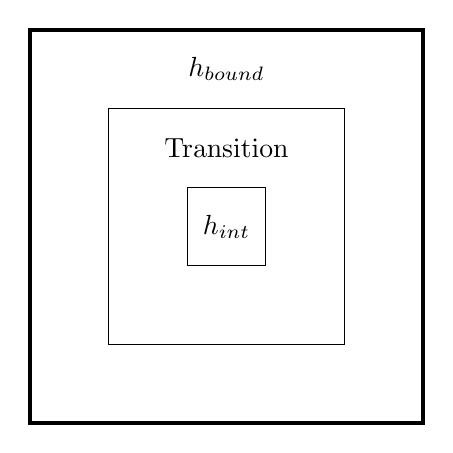
\begin{tikzpicture}
	\draw [line width = 0.5mm] (0,0) rectangle (5,5);
	\draw (1,1) rectangle (4,4);
	\draw (2,2) rectangle (3,3);
	\node[align=center] at (2.5, 2.5) {$h_{int}$};
	\node[align=center] at (2.5, 3.5) {Transition};
	\node[align=center] at (2.5, 4.5) {$h_{bound}$};
\end{tikzpicture}
\end{minipage}
\begin{minipage}[0.55]{0.49\linewidth}
Domain divided in three parts
\begin{itemize}
	\item Interior zone \\ $\to$ $h = h_{int} = 2^{-l}h_0$,
	\item Boundary zone \\ $\to$ $h = h_{bound} = 2^{-2l}h_0$,
	\item Intermediate zone \\ $\to$ $h = \Big(\frac{d}{(l + 3)\sigma}\Big)^2$.
\end{itemize}
\end{minipage}

\vspace{1cm}
\underline{Aim}. Order of convergence $O(\sqrt{h_{bound}}) = O(h_{int})$ saving computational time.
\end{frame}

\begin{frame} %%% Reflecting boundaries
\frametitle{Reflecting boundaries}
For all methods, equal treatment of reflecting boundaries. Consider $\partial D = \Gamma_r \cup \Gamma_k$ reflecting and killing boundaries.

\vspace{1cm}
\begin{minipage}[0]{0.4\linewidth}
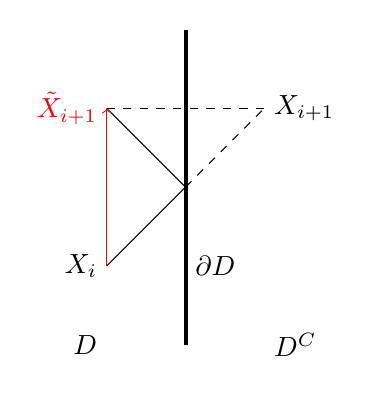
\begin{tikzpicture}
	\draw [line width = 0.5mm] (5,4) -- (5,0);
	\draw (4,1) -- (5,2);
	\draw [dashed] (5,2) -- (6,3);
	\draw (5,2) -- (4,3);
	\draw [dashed] (6,3) -- (4,3);
	\draw [->,color=red] (4,1) -- (4,3);
	\node [anchor=west] at (5,1) {$\partial D$};
	\node [anchor=east] at (4,1) {$X_i$};
	\node [anchor=west] at (6,3) {$X_{i+1}$};
	\node [anchor=east,color=red] at (4,3) {$\tilde X_{i+1}$};
	\node [anchor=east] at (4,0) {$D$};
	\node [anchor=west] at (6,0) {$D^C$};
\end{tikzpicture}
\end{minipage}
\begin{minipage}[0.4]{0.55\linewidth}
\begin{enumerate}
	\item Compute $X_{i+1}$;
	\item If the segment connecting $X_i$ and $X_{i+1}$ crosses $\Gamma_r$: \\
		$X_{i+1} \leftarrow \color{red}\tilde X_{i+1}$ reflection of $X_{i+1}$;
	\item If $\tilde X_{i+1} \notin D$: \\
		Check the segment connecting $X_i$ and $\tilde X_{i+1}$;
\end{enumerate}
\end{minipage}

\vspace{1cm}
This method does not spoil the order of convergence.
\end{frame}



